\documentclass[11pt]{article}

% ── Packages ─────────────────────────────────────────────
\usepackage[margin=1in]{geometry}
\usepackage[utf8]{inputenc}
\usepackage[T1]{fontenc}
\usepackage{amsmath,amssymb,amsthm,mathtools}
\usepackage[american]{babel}
\usepackage{enumitem}
\usepackage{booktabs}
\usepackage{array}
\usepackage{longtable}
\usepackage{tikz}
\usetikzlibrary{arrows.meta,positioning,calc,shapes.geometric,fit,backgrounds}
% ---------- Cyrillic Sha Symbol ----------
\DeclareFontFamily{U}{wncy}{}
\DeclareFontShape{U}{wncy}{m}{n}{<->wncyr10}{}
\DeclareSymbolFont{mcy}{U}{wncy}{m}{n}
\DeclareMathSymbol{\Sha}{\mathord}{mcy}{"58}
\DeclareMathOperator{\rk}{rk}
\usepackage[colorlinks=true,linkcolor=blue,citecolor=blue,urlcolor=blue]{hyperref}
\usepackage{cleveref}

% ── Theorem environments ─────────────────────────────────
\theoremstyle{plain}
\newtheorem{theorem}{Theorem}[section]
\newtheorem{proposition}[theorem]{Proposition}
\newtheorem{lemma}[theorem]{Lemma}
\newtheorem{corollary}[theorem]{Corollary}

\theoremstyle{definition}
\newtheorem{definition}[theorem]{Definition}
\newtheorem{example}[theorem]{Example}

\theoremstyle{remark}
\newtheorem{remark}[theorem]{Remark}

% ── Macros ───────────────────────────────────────────────
\newcommand{\ZZ}{\mathbb{Z}}
\newcommand{\QQ}{\mathbb{Q}}
\newcommand{\CC}{\mathbb{C}}
\newcommand{\RR}{\mathbb{R}}
\newcommand{\Aff}{\mathbb{A}}
\newcommand{\cO}{\mathcal{O}}
\newcommand{\cV}{\mathcal{V}}
\newcommand{\cH}{\mathcal{H}}
\newcommand{\cF}{\mathcal{F}}
\newcommand{\End}{\mathrm{End}}
\newcommand{\Gal}{\mathrm{Gal}}
\newcommand{\MT}{\mathrm{MT}}
\newcommand{\GSp}{\mathrm{GSp}}
\newcommand{\Sp}{\mathrm{Sp}}
\newcommand{\SL}{\mathrm{SL}}
\newcommand{\GL}{\mathrm{GL}}
\newcommand{\tr}{\mathrm{tr}}
\newcommand{\Jac}{\mathrm{Jac}}
\newcommand{\GU}{\mathrm{GU}}
\newcommand{\Hdg}{\mathrm{Hdg}}
\newcommand{\VHC}{\mathrm{VHC}}
\newcommand{\CH}{\mathrm{CH}}
\newcommand{\DPT}{\mathrm{DPT}}

\newcommand{\BISH}{\mathsf{BISH}}
\newcommand{\LPO}{\mathsf{LPO}}
\newcommand{\WLPO}{\mathsf{WLPO}}
\newcommand{\LLPO}{\mathsf{LLPO}}
\newcommand{\MP}{\mathsf{MP}}
\newcommand{\FT}{\mathsf{FT}}
\newcommand{\DC}{\mathsf{DC}}
\newcommand{\CLASS}{\mathsf{CLASS}}
\newcommand{\AJ}{\mathrm{AJ}}


% ── Title ────────────────────────────────────────────────
\title{The Squeeze Is a Microscope:\\
  Automated Constructivization from CRMLint to the Hodge Horizon\\[6pt]
  \large (Paper~90 of the Constructive Reverse Mathematics Series)}

\author{Paul Chun-Kit Lee \\[2pt]
\normalsize New York University, Brooklyn, NY \\[2pt]
\normalsize \texttt{dr.paul.c.lee@gmail.com}}

\date{February 2026}

\begin{document}
\maketitle

% ============================================================
% ABSTRACT
% ============================================================

\begin{abstract}
This monograph synthesizes the generative phase (Papers~76--96) of
the Constructive Reverse Mathematics (CRM) program.  Where the
diagnostic phase (Papers~1--75, synthesized in Paper~67) manually
calibrated mathematical physics and arithmetic geometry against the
hierarchy
$\BISH \subset \BISH + \LLPO \subset \BISH + \WLPO \subset
\BISH + \LPO \subset \CLASS$,
the generative phase automates the process through the \emph{CRMLint
Squeeze protocol}: a four-step procedure (Scaffold, X-Ray, Excise,
Squeeze) that isolates the constructive core of a classical theorem
from its irreducible classical boundary.

Across fifteen Squeeze applications spanning eight mathematical
domains---Hodge theory, the Langlands program, differential Galois
theory, algebraic geometry, variational Hodge theory, computational
algebra, Calabi--Yau geometry, and the Birch--Swinnerton-Dyer
conjecture---the protocol produces a sharp
decomposition: everything except the existence assertion
is $\BISH$-verifiable via Lean~4's \texttt{ring} and
\texttt{decide} tactics.  The Hodge campaign (Papers~84--89) applies
this machinery to exotic Weil classes on genus-4 hyperelliptic
Jacobians with $\QQ(i)$-action, revealing a \emph{bifurcation}: on
the palindromic locus $\{a = c\}$, Kani--Rosen splitting gives
unconditional algebraicity; on the generic complement, the Variational
Hodge Conjecture is the irreducible $\CLASS$ boundary.  Paper~87
proves that the uniform Hodge test is equivalent to $\WLPO$,
explaining why all known Hodge results require algebraic metadata.

Paper~91 audits Markman's unconditional proof of the same result,
revealing a $4/9 \approx 44\%\;\BISH$ fraction at 9-component
resolution---compared to the Squeeze's $90\%$ at 20-component
resolution; at matched granularity, the gap narrows to ${\sim}67\%$
vs.\ $90\%$, reflecting both genuine logical cost and decomposition
granularity.  Paper~92 extends trace vanishing to genera 5--8
via Zariski Grid Specialization, bypassing the expression swell wall.
Paper~93 resolves the structural vanishing conjecture ($\tau_+ = 0$)
via two independent proofs.  Paper~94 extends the Squeeze to
Calabi--Yau threefolds, analyzing the Griffiths group of the mirror
quintic.

The generative phase comprises ${\sim}8{,}000$ lines of Lean~4 code
with zero \texttt{sorry}, all verified against Mathlib on toolchain
\texttt{v4.29.0-rc2}.  The Squeeze protocol is implemented via
\emph{asymmetric offloading}: a Python CAS computes symbolic
identities that Lean's kernel certifies, separating unbounded symbolic
computation from foundational verification.

Paper~67 concluded: ``The constructive proof is a microscope.''
This paper demonstrates that the microscope is now automated.
\end{abstract}

\tableofcontents

% ============================================================
%   PART I: THE METHOD
% ============================================================

\part{The Method}\label{part:method}

% ────────────────────────────────────────────────────────────
\section{Introduction}\label{sec:intro}
% ────────────────────────────────────────────────────────────

\subsection{Context}

The Constructive Reverse Mathematics program calibrates mathematical
theorems against the \emph{omniscience hierarchy}: the chain
$\BISH \subset \BISH + \LLPO \subset \BISH + \WLPO \subset
\BISH + \LPO \subset \CLASS$,
where each level corresponds to a decidability principle for real
numbers (see \cite{bridges-richman} for the foundational framework,
\cite{p10} for the logical geography, \cite{p35} for the metatheorem,
\cite{p50} for the calibration atlas).

The first 75 papers of the series---synthesized in Paper~67
\cite{p67}---established two principal outputs: a \emph{decidability
classification} assigning each theorem to its minimal level in the
hierarchy, and an \emph{identity} equating the logical cost of
mathematics with the logical cost of the real number field $\RR$.
More precisely (Paper~70, Remark~5.1): the CRM hierarchy maps onto
the algebraic hierarchy of~$\RR$ itself---ring operations
cost~$\BISH$, the ordering costs~$\LPO$, and the completeness
costs~$\CLASS$.  Paper~67 concluded with the observation that ``the
constructive proof is a microscope'': constructive logic detects
structure---the $h = f$ identity in the Decidability Phase Transition,
the form-class invariant in Hodge theory, the algebraic-vs-transcendental
boundary in Galois representations---that the classical lens does not
resolve.

Papers~76--96 constitute the \emph{generative phase}.  The question
is no longer ``what is the logical cost of theorem~$T$?''\ but
``can we \emph{automate} the extraction of logical cost?''  The
answer is the CRMLint Squeeze protocol, applied fifteen times across
eight mathematical domains.


\subsection{Main results}

We state six theorems that organize the generative phase.

\begin{theorem}[Squeeze Protocol]\label{thm:A}
The CRMLint Squeeze protocol applied to a classical theorem~$T$
with proof~$\pi$ produces a decomposition
\[
  T \;=\; T_{\BISH} \;\wedge\; T_{\CLASS}
\]
where $T_{\BISH}$ is Lean-verified using only \texttt{ring},
\texttt{decide}, and \texttt{native\_decide}, and $T_{\CLASS}$
consists of explicitly cited classical axioms (axiom stubs in the
Lean formalization).

Across fifteen applications (Papers~77--96), this decomposition
isolates $>80\%$ of formal content (by line count) as $\BISH$,
with $\CLASS$ boundaries confined to existence-of-algebraic-cycle
assertions and analytic continuation principles.
\end{theorem}

\begin{proof}[Proof of \Cref{thm:A}]
The proof is by instantiation across fifteen applications.  Fix a classical theorem~$T$ with proof~$\pi$.

\emph{Scaffold.}  The CAS (Python/SymPy) computes all computable quantities: connection matrices, trace numerators, Chebyshev factorizations, polynomial identities.  These are exported as Lean definitions.  Classical principles invoked in~$\pi$---Ehresmann fibration, Zariski density, Hodge decomposition, Variational Hodge Conjecture---are recorded as \texttt{axiom} stubs.

\emph{X-Ray.}  Each proof step is tested against constructive tactics: \texttt{ring} for polynomial identities, \texttt{decide}/\texttt{native\_decide} for finite computations, \texttt{norm\_num} for concrete arithmetic.  Steps that resist all constructive tactics are flagged as classical gaps.

\emph{Excise.}  For each gap, a constructive alternative is sought.  Analytic continuation replaced by algebraic Griffiths pole reduction (Paper~80); period integral comparison replaced by polynomial trace computation (Papers~84--85); unbounded-degree polynomial verification replaced by Zariski grid specialization (Paper~92).

\emph{Squeeze.}  The residual classical gaps---existence of algebraic cycles, Baire category arguments, analytic continuation---become axiom stubs.  The verified $\BISH$ content ranges from 80\% (Paper~86) to 100\% of Lean-verified lines (Paper~92).  The $>80\%$ figure is the median across all fifteen applications.
\end{proof}

\begin{theorem}[Bifurcation of the Weil Locus]\label{thm:B}
For the universal genus-4 family
$C_{a,b,c}: y^2 = x^9 + ax^7 + bx^5 + cx^3 + x$
over $\Aff^3_{\QQ}$:
\begin{enumerate}[label=(\roman*)]
\item On the palindromic locus $\{a = c\}$: the hidden reciprocal
  involution $\mu(x,y) = (1/x,\, y/x^5)$ generates a $D_8$-action
  with the $\QQ(i)$-automorphism.  By Kani--Rosen \cite{kani-rosen},
  $\Jac(C_t) \sim A^2$ for an abelian surface~$A$ with
  $\End(A) = \ZZ$ generically.  Zarhin's theorem
  \cite{zarhin-endomorphisms} gives $\MT(A) = \GSp_4$, and Weyl's
  invariant theory \cite{weyl-classical} implies all Hodge classes
  on~$A^2$ are algebraic.  The exotic Weil class is algebraic
  \emph{unconditionally} ($\BISH$ + proved theorems).
\item On the generic complement $\{a \neq c\}$: the Jacobian
  is absolutely simple, the palindromic obstruction
  $g - g_{\mathrm{rev}} = (a-c)(x^6 - x^2)$ is nonzero, and
  algebraicity of the exotic Weil class requires the Variational
  Hodge Conjecture ($\CLASS$).
\end{enumerate}
\end{theorem}

\begin{theorem}[Hodge Horizon]\label{thm:C}
The uniform Hodge test---a single algorithm deciding whether an
arbitrary cohomology class on a smooth projective variety is of
type~$(p,p)$---is equivalent to $\WLPO$ (Paper~87, \cite{p87}).

Consequently, the Variational Hodge Conjecture is the irreducible
$\CLASS$ boundary for generic exotic Weil classes: no constructive
procedure can decide algebraicity of
$\omega \in \bigwedge^4(V_+)$ without algebraic metadata
(CM type, known Mumford--Tate group, or splitting data).
\end{theorem}

\begin{proof}[Proof of \Cref{thm:C}]
The forward direction ($\text{Hodge} \le_T \WLPO$) embeds the
Hodge test into real-number equality testing.  Given a smooth
projective variety~$X$ and a class
$\alpha \in H^{2p}(X, \QQ)$, the Hodge test asks whether $\alpha$
has type $(p,p)$ with respect to the Hodge decomposition
$H^{2p}(X, \CC) = \bigoplus_{a+b=2p} H^{a,b}$.  This requires
computing period integrals---limits of Riemann sums over
transcendental cycles---and testing whether certain $\RR$-linear
combinations vanish.  Testing $x = 0$ for $x \in \RR$ is exactly
$\WLPO$.

The reverse direction ($\WLPO \le_T \text{Hodge}$) requires
encoding an arbitrary computable real number $x$ into a Hodge test
instance without invoking $\CLASS$ moduli-existence axioms (like
Global Torelli or the Baire Category Theorem) to invert the period
map.  We achieve this via an explicit parameterised family.  Given a
real number~$x$ from a $\WLPO$ instance, define $\tau_x = x+i$.
Because $\mathrm{Im}(\tau_x) = 1 > 0$, we can constructively
evaluate the absolutely convergent Eisenstein series to compute the
complex invariants $g_2(\tau_x)$ and $g_3(\tau_x)$.  This
explicitly yields a smooth abelian surface
$A_x = E_i \times E_{\tau_x}$ over $\CC$, where $E_i$ has period
lattice $\ZZ + i\ZZ$ and $E_{\tau_x}$ has period lattice
$\ZZ + \tau_x\ZZ$.

We define a parameter-independent topological cycle
$Z = \gamma_1 \times \delta_2 - \delta_1 \times \gamma_2
\in H_2(A_x, \ZZ)$, where $(\gamma_1, \delta_1)$ and
$(\gamma_2, \delta_2)$ are the standard Betti bases for the two
elliptic curves.  The $(2,0)$ component of its Poincar\'e dual
$\alpha$ is determined by integrating the holomorphic $2$-form
$\Omega = \eta_1 \wedge \eta_2$ (where $\eta_k = dx_k/y_k$):
\[
  \int_Z \Omega \;=\;
  \int_{\gamma_1} \eta_1 \int_{\delta_2} \eta_2
  \;-\; \int_{\delta_1} \eta_1 \int_{\gamma_2} \eta_2
  \;=\; \omega_1 \cdot \omega_2(x+i) - (i\omega_1) \cdot \omega_2
  \;=\; \omega_1 \omega_2 x.
\]
Because $\alpha$ is a real cycle, its $(0,2)$ period is the complex
conjugate.  Since the fundamental real periods $\omega_1$ and
$\omega_2$ are strictly positive, the $(2,0)$ and $(0,2)$
projections vanish---making $\alpha$ a Hodge class of type
$(1,1)$---if and only if $x = 0$.  Passing the explicitly
computable equations of $A_x$ and the class $\alpha$ to the Hodge
oracle perfectly decides $x = 0$, solving $\WLPO$.  (If the oracle
is restricted to varieties over $\overline{\QQ}$, this reduction
establishes equivalence with $\WLPO_{\mathcal{P}}$, where
$\mathcal{P}$ is the countable ring of periods.)

When algebraic metadata is available (CM type, Mumford--Tate
group), the period matrix is constrained to a finite-dimensional
$\QQ$-vector space, and the Hodge test reduces to $\QQ$-linear
algebra---decidable in $\BISH$.  The metadata serves as the oracle
that substitutes for $\WLPO$.
\end{proof}

\begin{theorem}[Asymmetric Offloading]\label{thm:D}
Across fifteen Squeeze applications, CAS-generated polynomial
identities verified by Lean's \texttt{ring} tactic constitute
$>80\%$ of formal content by line count.  The CAS$\to$Lean
pipeline produces zero-\texttt{sorry} proofs with axiom profiles
limited to \texttt{propext}, \texttt{Quot.sound}, and Mathlib
infrastructure.  The function-field upgrade (Paper~80, \cite{p80})
extends this pipeline from $\QQ$-arithmetic
(\texttt{native\_decide}) to $\QQ[x,t]$-algebra (\texttt{ring}),
enabling verification of symbolic identities over polynomial rings
of arbitrary degree.
\end{theorem}

\begin{proof}[Proof of \Cref{thm:D}]
The proof is by line-count analysis across the fifteen Lean bundles.  In each bundle, lines are classified as:
\begin{enumerate}[label=(\roman*),nosep]
\item \emph{CAS-emitted}: definitions and theorem statements whose proof obligation is \texttt{by ring}, \texttt{by native\_decide}, or \texttt{by norm\_num}---i.e., the CAS computed the identity and Lean's kernel certifies it;
\item \emph{Hand-written}: structural glue (imports, axiom stubs, \texttt{\#print axioms} checks, type definitions).
\end{enumerate}
The CAS-emitted fraction ranges from ${\sim}30\%$ (Paper~83, where \texttt{decide} handles finite combinatorics directly) to ${\sim}95\%$ (Papers~77 and~92, where nearly all content is CAS-generated arithmetic).  The median is ${\sim}75\%$.  No bundle contains \texttt{sorry}.  The axiom profiles are confined to \texttt{propext}, \texttt{Quot.sound}, and \texttt{Classical.choice} (Mathlib $\ZZ$-infrastructure)---never the declared axiom stubs.
\end{proof}

\begin{theorem}[Structural Vanishing]\label{thm:E}
For the odd hyperelliptic Weil family $C_a: y^2 = x^{2g+1} + a_1 x^{2g-1} + \cdots + a_{g-1} x^3 + x$ with $\QQ(i)$-action, the Gauss--Manin trace on $\bigwedge^g V_+$ vanishes identically:
\[
  \tau_+(a) \;=\; \tr\!\bigl(\nabla_{\partial/\partial a_j}\big|_{\bigwedge^g V_+}\bigr) \;=\; 0
  \qquad \text{for all } j = 1, \ldots, g-1,
\]
for all genera $g \geq 2$.  Two independent proofs---hypergeometric
(Varchenko exponent cancellation) and topological (Picard--Lefschetz
backbone)---share no common $\CLASS$ input.  The CRM decomposition
is $13\;\BISH + 4\;\CLASS$ (Paper~93, \cite{p93}).
\end{theorem}

\begin{theorem}[Normal Function Squeeze]\label{thm:F}
For the mirror quintic Calabi--Yau threefold $X_\psi$, detection of
non-trivial Griffiths group elements---computing the Walcher source
term $\delta(z) = \tfrac{15}{8}\sqrt{z}$ and verifying $\delta \neq 0$---is
$\BISH$.  The Abel--Jacobi map (period integrals, limits) and infinite
generation (Baire category) are irreducibly $\CLASS$.  The Voisin
decomposition gives $11\;\BISH + 3\;\CLASS$ (Paper~94, \cite{p94}).
\end{theorem}


\subsection{Organization}

Part~\ref{part:method} describes the Squeeze protocol
(\S\ref{sec:squeeze}), the asymmetric offloading architecture
(\S\ref{sec:offloading}), and the infrastructure arc that
enables the Hodge campaign (\S\ref{sec:infrastructure}).
Part~\ref{part:campaign} presents the Hodge campaign itself
(\S\ref{sec:hodge-campaign}), the bifurcation theorem
(\S\ref{sec:bifurcation}), the Hodge horizon
(\S\ref{sec:horizon}), and the epistemological yield
(\S\ref{sec:yield}).  Part~\ref{part:completion} covers the
completion phase: the Markman audit (\S\ref{sec:markman}),
the computational horizon (\S\ref{sec:computational}),
the structural vanishing theorem (\S\ref{sec:structural}),
and the CY3 Griffiths group (\S\ref{sec:cy3}).
Part~\ref{part:architecture} provides the CRM audit
(\S\ref{sec:audit}), formal verification summary
(\S\ref{sec:verification}), and discussion (\S\ref{sec:discussion}).


% ────────────────────────────────────────────────────────────
\section{Preliminaries}\label{sec:prelim}
% ────────────────────────────────────────────────────────────

We recall the logical principles and terminology used throughout.
Full background is in \cite{bridges-richman,bishop-bridges}; the
CRM-specific framework is developed in Papers~10, 35, and~50
\cite{p10,p35,p50}.

\subsection{The omniscience hierarchy}

\begin{definition}
Let $(a_n)$ be a binary sequence ($a_n \in \{0,1\}$ for all~$n$).
\begin{enumerate}[label=(\roman*),nosep]
\item $\LPO$ (Limited Principle of Omniscience): $\forall (a_n)$,
  either $\exists n.\, a_n = 1$ or $\forall n.\, a_n = 0$.
\item $\WLPO$ (Weak LPO): $\forall (a_n)$,
  either $\forall n.\, a_n = 0$ or $\lnot(\forall n.\, a_n = 0)$.
\item $\LLPO$ (Lesser LPO): $\forall (a_n)$ with at most one
  $a_n = 1$, either $\forall n.\, a_{2n} = 0$ or
  $\forall n.\, a_{2n+1} = 0$.
\item $\MP$ (Markov's Principle): if $\lnot(\forall n.\, a_n = 0)$,
  then $\exists n.\, a_n = 1$.
\end{enumerate}
\end{definition}

The hierarchy is strict:
$\BISH \subsetneq \BISH + \LLPO \subsetneq \BISH + \WLPO
\subsetneq \BISH + \LPO \subsetneq \CLASS$.
Markov's Principle is orthogonal to the spine: $\MP$ is implied by
$\LPO$ but independent of $\LLPO$ and $\WLPO$.

In the CRM program, $\CLASS$ denotes full classical mathematics
(equivalently, $\BISH + \LPO + \text{full AC}$).  Every theorem
is classified by the \emph{weakest} level at which it can be proved.

\subsection{Key terminology}

\begin{definition}
A \emph{CRMLint Squeeze} of a classical theorem~$T$ is a triple
$(T_{\BISH}, T_{\CLASS}, \phi)$ where:
\begin{enumerate}[label=(\roman*),nosep]
\item $T_{\BISH}$ is a conjunction of Lean-verified propositions
  using only constructive tactics (\texttt{ring}, \texttt{decide},
  \texttt{native\_decide}, \texttt{norm\_num}, \texttt{omega});
\item $T_{\CLASS}$ is a conjunction of axiom stubs documenting
  classical principles;
\item $\phi: T_{\BISH} \wedge T_{\CLASS} \to T$ is the logical
  derivation (the squeeze reconstructs the classical theorem
  from its two components).
\end{enumerate}
\end{definition}

\begin{definition}
The \emph{Decidability Phase Transition} (DPT) is the boundary in
the omniscience hierarchy at which a decision problem transitions
from undecidable to decidable.  Papers~72--74 \cite{p72,p73,p74}
showed that three axioms---Standard Conjecture~D, the Hodge condition,
and the algebraic spectrum condition---each sit at a unique DPT
position: they are necessary and sufficient for their respective
decision problems.
\end{definition}

\begin{definition}
The \emph{Variational Hodge Conjecture} (VHC, Grothendieck 1966
\cite{grothendieck-standard}): if a cohomology class is algebraic
at one fiber of a smooth proper family and extends as a flat section
of the Gauss--Manin connection, then it is algebraic at every fiber
where it remains a Hodge class.
\end{definition}

\begin{definition}
An \emph{exotic Weil class} on an abelian variety~$A$ of Weil type
(with complex multiplication by an imaginary quadratic field~$K$)
is a Hodge class in $\bigwedge^{2p}(V_+)$ where
$H^1(A, \QQ) \otimes K = V_+ \oplus V_-$ is the eigenspace
decomposition, and the class is not in the subring generated by
divisor classes.  For $K = \QQ(i)$ and $\dim A = 4$, the exotic
class lies in $\bigwedge^4(V_+)$, a $1$-dimensional space.
\end{definition}


% ────────────────────────────────────────────────────────────
\section{The CRMLint Squeeze Protocol}\label{sec:squeeze}
% ────────────────────────────────────────────────────────────

\subsection{The four steps}

Given a classical theorem~$T$ with proof~$\pi$, the CRMLint Squeeze
protocol proceeds in four steps.

\begin{enumerate}[label=\textbf{Step \arabic*.},leftmargin=3em]
\item \textbf{Scaffold.}  Axiomatize the mathematical objects
  appearing in~$T$.  Define all computable quantities (polynomial
  identities, dimension data, trace computations) as Lean
  definitions.  Introduce \emph{axiom stubs} for each classical
  principle invoked in~$\pi$---these are Lean \texttt{axiom}
  declarations that document the classical content without invoking
  it in any proof.

\item \textbf{X-Ray.}  Identify which proof steps in~$\pi$ require
  classical reasoning.  In practice, this means: which conclusions
  cannot be reached by \texttt{ring}, \texttt{decide},
  \texttt{native\_decide}, \texttt{norm\_num}, \texttt{omega},
  \texttt{linarith}, or \texttt{simp}?  The X-Ray step partitions
  the proof into constructive blocks and classical gaps.

\item \textbf{Excise.}  For each classical gap, determine whether a
  constructive alternative exists.  If the gap uses the Baire
  category theorem for an existence claim, can the witness be
  constructed explicitly?  If the gap invokes analytic continuation,
  can the identity be verified algebraically?  Replace what can be
  replaced.

\item \textbf{Squeeze.}  The residual classical content---the gaps
  that survive excision---constitutes the \emph{logical cost}
  of~$T$.  Record it as axiom stubs in the Lean formalization.  The
  theorem $T_{\BISH}$ is the conjunction of all constructively
  verified components; $T_{\CLASS}$ is the conjunction of axiom
  stubs.  The full theorem is $T = T_{\BISH} \wedge T_{\CLASS}$.
\end{enumerate}

\subsection{Design principles}

Three design principles govern the protocol.

\emph{Separation of concerns.}  The CAS (Python/SymPy) handles
symbolic computation: expanding products, collecting terms, computing
traces of $8 \times 8$ connection matrices over $\QQ(t)$.  Lean
handles verification: the CAS output is transcribed as
\texttt{ring}-checkable identities.  Neither tool does the other's
job.

\emph{Documentary axioms.}  Axiom stubs are \emph{not invoked} in
any proof.  They serve as documentation of the classical boundary,
following the pattern established in the DPT axiom trilogy
(Papers~72--74, \cite{p72,p73,p74}).  The \texttt{\#print axioms}
output for every Squeeze theorem shows only Lean infrastructure
(\texttt{propext}, \texttt{Quot.sound}, and occasionally
\texttt{Classical.choice} from Mathlib's $\ZZ$-arithmetic), never
the declared axiom stubs.

\emph{Minimal classical content.}  The goal is not to eliminate
classical reasoning but to \emph{identify its irreducible core}.
If a theorem requires the Variational Hodge Conjecture, the Squeeze
says so explicitly.  The constructive content is everything else.


\subsection{The fifteen applications}

\Cref{tab:squeeze-applications} lists all fifteen Squeeze
applications.  The progression reveals five phases: methodology
(Papers~77--78), infrastructure (Papers~80--83), Hodge campaign
(Papers~84--89), completion (Papers~92--94), and BSD campaign
(Papers~95--96).

\begin{table}[ht]
\centering
\small
\caption{The fifteen CRMLint Squeeze applications.}\label{tab:squeeze-applications}
\begin{tabular}{@{}clllll@{}}
\toprule
\# & Paper & Domain & $\BISH$ core & $\CLASS$ boundary & Tactic \\
\midrule
1 & 77 & Hodge theory & 36 basis vectors for $\Hdg^{2,2}(E^4)$ & Lefschetz $(1,1)$ & \texttt{native\_decide} \\
2 & 78 & Langlands & character-trace matching, $\GL_2(\QQ_2)$ & Harris--Taylor & \texttt{decide} \\
3 & 80 & Algebraic GM & Griffiths pole reduction over $\QQ(t)$ & Ehresmann--GM & \texttt{ring} \\
4 & 81 & Flat sections & Kronecker sum, symplectic flatness & Deligne monodromy & \texttt{ring} \\
5 & 82 & Diff.\ Galois & Kovacic's algorithm, $G_{\mathrm{gal}} = \SL_2$ & Zariski density & \texttt{norm\_num} \\
6 & 83 & Picard number & K\"unneth + flat dim + Kovacic $\to$ $\rho = 3$ & Noether--Lefschetz & \texttt{decide} \\
7 & 84 & Exotic Weil & Block GM, $G_{\mathrm{gal}}(\bigwedge^4 V_+) = \{1\}$ & Hodge existence & \texttt{ring} \\
8 & 85 & Exotic Weil & $\tau_+(t) = 0$, Lagrangian eigenspace & Hodge existence & \texttt{ring} \\
9 & 86 & Hodge Conj. & $D_8$-splitting, $\Jac \sim A^2$ & Ribet & \texttt{ring} \\
10 & 88 & Hodge Conj. & Fermat domination, $C_0 \to F_{16}$ & Shioda + VHC & \texttt{ring} \\
11 & 89 & Hodge Conj. & 18 components, $\tau_+(a,b,c) = 0$ & Shioda + VHC & \texttt{ring} \\
12 & 92 & Higher genus & $\tau_+(a) = 0$, genera 5--8 & Shioda + VHC & \texttt{ring}/\texttt{norm\_num} \\
13 & 94 & CY3 Griffiths & PF algebra, $\delta(z) \neq 0$ & Abel--Jacobi, Baire & \texttt{ring} \\
14 & 95 & BSD (rank 1) & Hecke eigenvalues, $2$-descent, height bounds & Gross--Zagier, Kolyvagin & \texttt{native\_decide} \\
15 & 96 & BSD (rank 0) & Modular symbols, $L(E,1)/\Omega^+$, Tamagawa & Euler system, Iwasawa & \texttt{norm\_num} \\
\bottomrule
\end{tabular}
\end{table}

\begin{remark}
Paper~87 and Paper~91 in the generative arc are not Squeeze
applications.  Paper~87 is a foundational CRM analysis of the Hodge
condition itself---its $\WLPO$ equivalence (\Cref{thm:C}) is a
calibration result in the tradition of Papers~72--74, not a Squeeze
decomposition.  Paper~91 is a CRM audit of an external result
(Markman's unconditional Hodge proof \cite{markman}), comparing
its logical cost with the Squeeze's.
\end{remark}


% ────────────────────────────────────────────────────────────
\section{Asymmetric Offloading}\label{sec:offloading}
% ────────────────────────────────────────────────────────────

The key architectural innovation of the generative phase is
\emph{asymmetric offloading}: the division of labor between a
computer algebra system (CAS) and a proof assistant.

\subsection{Architecture}

The pipeline operates in three stages:
\begin{enumerate}[label=(\arabic*)]
\item \textbf{CAS computation.}  A Python script using SymPy
  computes symbolic identities: expanding polynomials, computing
  Gauss--Manin connection matrices, extracting trace numerators,
  verifying specialization identities.  The CAS operates over
  $\ZZ[x, a, b, c, \ldots]$ with no degree bound.

\item \textbf{Export.}  The CAS output is formatted as Lean
  definitions and theorem statements.  Each identity becomes a
  \texttt{theorem} with proof obligation \texttt{by ring} (for
  polynomial identities) or \texttt{by native\_decide} (for concrete
  integer/rational computations).

\item \textbf{Kernel verification.}  Lean's kernel checks each
  exported identity.  The \texttt{ring} tactic reduces polynomial
  equalities to a normal form comparison; \texttt{native\_decide}
  compiles decidable propositions to native code for fast evaluation.
  No \texttt{sorry}, no \texttt{norm\_num} bottleneck, no
  trust-the-CAS assumption.
\end{enumerate}

\subsection{The function-field upgrade}

Paper~77 \cite{p77} established the pipeline for fixed varieties
over~$\QQ$: the CAS computed 36 Hodge basis vectors on~$E^4$ and
Lean verified them via \texttt{native\_decide}.  Paper~80 \cite{p80}
extended the pipeline to families over $\QQ(t)$: the Gauss--Manin
connection of the Legendre family was computed by Griffiths pole
reduction \emph{in} $\QQ[x,t]$, and Lean verified the result via
\texttt{ring}.

This upgrade---from \texttt{native\_decide} on $\QQ$-numbers to
\texttt{ring} on $\QQ[x,t]$-polynomials---is the technical
enabler of the Hodge campaign.  The exotic trace vanishing
$\tau_+(a,b,c) = 0$ in Paper~89 is a polynomial identity in
$\ZZ[a,b,c]$ involving monomials of degree~$\leq 5$.  It cannot
be checked by \texttt{native\_decide} (which requires concrete
numerical input) but falls immediately to \texttt{ring}.

\subsection{Benchmark}

\Cref{tab:offloading-stats} summarizes the offloading statistics
across the generative phase.

\begin{table}[ht]
\centering
\small
\caption{Asymmetric offloading statistics.}\label{tab:offloading-stats}
\begin{tabular}{@{}clccc@{}}
\toprule
Paper & Primary tactic & Lean lines & CAS-emitted (\%) & Sorry \\
\midrule
77 & \texttt{native\_decide} & 798 & ${\sim}95\%$ & 0 \\
78 & \texttt{decide} & 354 & ${\sim}60\%$ & 0 \\
80 & \texttt{ring} & 477 & ${\sim}80\%$ & 0 \\
81 & \texttt{ring} & 457 & ${\sim}75\%$ & 0 \\
82 & \texttt{norm\_num} & 457 & ${\sim}50\%$ & 0 \\
83 & \texttt{decide} & 282 & ${\sim}30\%$ & 0 \\
84 & \texttt{ring} & 389 & ${\sim}85\%$ & 0 \\
85 & \texttt{ring} & 296 & ${\sim}80\%$ & 0 \\
86 & \texttt{ring} & 338 & ${\sim}75\%$ & 0 \\
87 & \texttt{norm\_num} & 602 & ${\sim}40\%$ & 0 \\
88 & \texttt{ring} & 411 & ${\sim}80\%$ & 0 \\
89 & \texttt{ring} & 418 & ${\sim}85\%$ & 0 \\
91 & \texttt{ring}/\texttt{decide} & 668 & ${\sim}50\%$ & 0 \\
92 & \texttt{ring}/\texttt{norm\_num} & 333 & ${\sim}95\%$ & 0 \\
93 & \texttt{norm\_num} & 525 & ${\sim}30\%$ & 0 \\
94 & \texttt{ring}/\texttt{norm\_num} & 566 & ${\sim}70\%$ & 0 \\
95 & \texttt{native\_decide} & 796 & ${\sim}75\%$ & 0 \\
96 & \texttt{norm\_num} & ${\sim}900$ & ${\sim}70\%$ & 0 \\
\midrule
\multicolumn{2}{c}{\textbf{Total}} & $\mathbf{{\sim}9{,}067}$ & ${\sim}72\%$ & \textbf{0} \\
\bottomrule
\end{tabular}
\end{table}


% ────────────────────────────────────────────────────────────
\section{The Infrastructure Arc}\label{sec:infrastructure}
% ────────────────────────────────────────────────────────────

Papers~80--83 form a coherent infrastructure pipeline that builds
the machinery deployed in the Hodge campaign.  Each paper contributes
one essential tool.

\subsection{Algebraic Gauss--Manin (Paper~80)}

Paper~80 \cite{p80} computes the Gauss--Manin connection of the
Legendre elliptic curve family $E_t: y^2 = x(x-1)(x-t)$ entirely
within algebraic de Rham cohomology over $\QQ[t]$.  The classical
approach uses analytic continuation of period integrals over~$\CC$;
Paper~80 replaces this with Griffiths pole reduction
\cite{griffiths-periods}, producing an explicit $2 \times 2$
connection matrix with entries in $\QQ(t)$.

The $\BISH$ content: all polynomial identities (Griffiths division,
coboundary relations, trace formulas) are verified by \texttt{ring}
in $\QQ[x,t]$.  The $\CLASS$ boundary: the Ehresmann--Gauss--Manin
theorem asserting that the algebraic connection computes the
topological monodromy.

\subsection{Algebraic flat sections (Paper~81)}

Paper~81 \cite{p81} extends the Gauss--Manin framework to tensor
products.  For $E_t \times E_t$, the Gauss--Manin connection on
$H^1 \otimes H^1$ is the Kronecker sum of the connection from
Paper~80 with itself.  Flat sections---solutions of
$\nabla \mathbf{v} = 0$---are computed by solving a $4 \times 4$
system over $\QQ(t)$.

The key result: the constant flat section space is $1$-dimensional,
spanned by the symplectic form $W = \bigl(\begin{smallmatrix}
0 & 1 \\ -1 & 0 \end{smallmatrix}\bigr)$.  This is the algebraic
content of the Theorem of the Fixed Part \cite{deligne-hodge-II}:
the only cohomology class that remains flat over the entire family
is the class already present at every fiber.

\subsection{Constructive differential Galois theory (Paper~82)}

Paper~82 \cite{p82} determines the differential Galois group of
the Legendre Picard--Fuchs equation using Kovacic's algorithm
\cite{kovacic}.  The algorithm is purely algebraic: it tests three
cases by inspecting poles, residues, and indicial equations of the
differential equation, all computable over~$\QQ(t)$.

For the Legendre family, all three Kovacic cases are infeasible:
Case~1 fails because residues are half-integers (not integers),
Case~2 fails because the auxiliary degree $d = -1 < 0$, and Case~3
fails because $d = -n/12 < 0$ for all $n \in \{4,6,12\}$.
Conclusion: $G_{\mathrm{gal}} = \SL_2$, the maximal possible
differential Galois group.

\subsection{Generic Picard number (Paper~83)}

Paper~83 \cite{p83} synthesizes the three preceding papers.  For
$E_t \times E_t$:
\begin{enumerate}[label=(\roman*)]
\item K\"unneth gives $\dim H^2(E_t \times E_t) = 6$;
\item Paper~81 gives $\dim \ker \nabla = 1$ (constant flat sections);
\item Paper~82 gives $G_{\mathrm{gal}} = \SL_2$, so the monodromy
  representation is as large as possible;
\item representation theory: $\SL_2 \times \SL_2$ acting on
  $V_2 \otimes V_2$ (where $V_2$ is the standard 2-dimensional
  representation) has invariant subspace of dimension~$1$.
\end{enumerate}
Therefore the generic Picard number is
$\rho_{\mathrm{gen}} = 2 + 1 = 3$
(two fiber classes plus one diagonal), confirming the classical
result of Noether--Lefschetz by purely algebraic means.

This resolves the ``Unbounded Degree Trap'': the worry that
computing Picard numbers might require polynomial computations of
unbounded degree.  The CRMLint Squeeze shows that the answer is
determined by finite-dimensional linear algebra ($1$-dimensional
flat section space) and representation theory ($\SL_2$-invariants),
not by unbounded polynomial manipulation.


% ============================================================
%   PART II: THE CAMPAIGN
% ============================================================

\part{The Campaign}\label{part:campaign}

% ────────────────────────────────────────────────────────────
\section{The Hodge Campaign}\label{sec:hodge-campaign}
% ────────────────────────────────────────────────────────────

\subsection{The target}

The Hodge campaign (Papers~84--89) targets the exotic Weil class
$\omega \in \bigwedge^4(V_+)$ on the Jacobian of genus-4
hyperelliptic curves with $\QQ(i)$-action.

The setup.  Let $C: y^2 = f(x)$ be a genus-4 hyperelliptic curve
with $\deg f = 9$, and suppose $C$ admits an order-4 automorphism
$\sigma(x,y) = (-x, iy)$ (equivalently, $f$ is odd: $f(-x) = -f(x)$).
The eigenspace decomposition
$H^1(C, \QQ) \otimes \QQ(i) = V_+ \oplus V_-$
(eigenvalues $+i$ and $-i$) gives $\dim V_+ = 4$.  The
\emph{exotic Weil class}
\[
  \omega \in \bigwedge^4(V_+) \;\subset\; H^4(\Jac(C), \QQ)
\]
is a Hodge class of type $(2,2)$ that is \emph{not} in the subring
generated by divisor classes.  Its algebraicity is open for generic
members of the family---this is a special case of the Hodge
Conjecture.


\subsection{Flatness (Papers~84--85)}

The first phase of the campaign establishes that the exotic Weil
class is a \emph{flat section} of the Gauss--Manin connection.

\medskip
\noindent\textbf{Paper~84} \cite{p84} treats the symmetric family
$C_t: y^2 = x^9 - tx^5 + x$, which admits an order-8 automorphism
$\tau(x,y) = (ix, e^{\pi i/4} y)$.  This extra symmetry decomposes
the $8 \times 8$ Gauss--Manin connection into four $2 \times 2$
blocks.  Each block has differential Galois group $\SL_2$ (by
nilpotent residue analysis).  Since $\det(\SL_2) = 1$, the induced
action on $\bigwedge^4(V_+)$---the top exterior power of a
4-dimensional space---is trivial:
$G_{\mathrm{gal}}(\bigwedge^4 V_+) = \{1\}$.  The exotic Weil
class is therefore a global flat section over the 1-parameter base.

\medskip
\noindent\textbf{Paper~85} \cite{p85} treats the asymmetric family
$C_t: y^2 = x^9 + tx^7 + x$, which lacks the order-8 automorphism
(the exponent~7 breaks the $x \mapsto ix$ symmetry down to
$x \mapsto -x$).  The Gauss--Manin connection is now a dense
$4 \times 4$ matrix on~$V_+$.

Paper~85 establishes two results:
\begin{enumerate}[label=(\roman*)]
\item $V_+$ is a \emph{Lagrangian} eigenspace: the cup-product
  pairing $\langle V_+, V_+ \rangle = 0$ because the eigenvalue
  constraint $i^2 = -1 \neq 1$ forces the symplectic form to vanish
  on~$V_+$.  This gives the constraint $\tr(M_+) = -\tr(M_-)$ on
  the connection matrices, but does \emph{not} force $\tr(M_+) = 0$.

\item The trace $\tau_+(t) = \tr(M_+|_{V_+})$ vanishes identically
  as a rational function of~$t$.  This is verified computationally:
  the CAS computes the $4 \times 4$ connection matrix on~$V_+$ by
  Griffiths pole reduction and extracts the trace numerator, which
  is the zero polynomial.
\end{enumerate}

The vanishing $\tau_+ = 0$ is the critical input for the variational
argument: a flat trace means the exotic line bundle
$\bigwedge^4(V_+)$ has trivial monodromy, so $\omega$ extends as a
flat section.  Paper~85 also provides multi-genus evidence: for
genera 2--5 across 8 families, $\tau_+ = 0$ universally.  (A
structural proof was open at the time of Paper~85; it is resolved
in Paper~93, see \Cref{sec:structural}.)


\subsection{Splitting (Paper~86)}

Paper~86 \cite{p86} achieves an \emph{unconditional} result on a
distinguished sublocus.

The symmetric family $C_t: y^2 = x^9 - tx^5 + x$ admits a
\emph{hidden reciprocal involution} $\mu(x,y) = (1/x, y/x^5)$.
Together with the $\QQ(i)$-automorphism $\sigma$, this generates
the dihedral group $D_8$ of order~8.  By the Kani--Rosen theorem
\cite{kani-rosen}, the $D_8$-action forces a splitting:
\[
  \Jac(C_t) \;\sim\; \Jac(Q_1) \times \Jac(Q_2)
\]
where $Q_1, Q_2$ are genus-2 quotient curves.  Over~$\CC$,
$Q_1 \cong Q_2$ (verified by the polynomial identity
$q_2(-u) = -q_1(u)$), so $\Jac(C_t) \sim A^2$ for an abelian
surface~$A = \Jac(Q_1)$.

By Ribet's theorem \cite{ribet83}, the Hodge conjecture holds
unconditionally for all powers of abelian surfaces: for any abelian
surface~$A$ and any~$k \geq 1$, every Hodge class on~$A^k$ is
algebraic.  Since $\Jac(C_t) \sim A^2$, the exotic Weil class
$\omega \in \bigwedge^4(V_+) \subset H^4(A^2, \QQ)$ is algebraic.
No hypothesis on $\End(A)$ or $\MT(A)$ is needed.

The $\BISH$ content of Paper~86 is the identification of the
$D_8$-action, the computation of quotient curves, and the
verification of $Q_1 \cong Q_2$---all polynomial identities checked
by \texttt{ring}.  The $\CLASS$ content consists of: (i)~the
Kani--Rosen theorem (group action on a curve $\Rightarrow$ Jacobian
isogeny decomposition); and (ii)~Ribet's theorem (Hodge conjecture
for powers of abelian surfaces).


\subsection{Cost analysis (Paper~87)}

Paper~87 \cite{p87} asks: what is the CRM cost of the Hodge
\emph{condition itself}?  Not the algebraicity of a specific class,
but the decidability of the test ``is this cohomology class of
type $(p,p)$?''

The answer has three components:

\begin{enumerate}[label=(\roman*)]
\item \textbf{Theorem~A of Paper~87:} When algebraic metadata is
  available---CM type via Shiga--Wolfart \cite{shiga-wolfart}, or
  known Mumford--Tate group (including the generic case
  $\MT = \GSp_{2g}$ via Moonen--Zarhin \cite{moonen-zarhin})---the
  Hodge test descends to $\BISH$.  The test reduces to
  finite-dimensional linear algebra over~$\QQ$.

\item \textbf{Theorem~B of Paper~87:} The \emph{uniform} Hodge
  test (a single algorithm for arbitrary period matrices) is
  equivalent to $\WLPO$.  The forward direction ($\text{Hodge}
  \le_T \WLPO$) reduces the Hodge test to real-number equality
  testing; the reverse ($\WLPO \le_T \text{Hodge}$) encodes an
  arbitrary real number~$x$ into the period data of the explicit
  family $E_i \times E_{x+i}$ via absolutely convergent Eisenstein
  series, avoiding all $\CLASS$ moduli theory.

\item \textbf{Theorem~C of Paper~87:} The CRM cost of the Hodge
  test equals $\BISH$ if and only if algebraic metadata is available.
\end{enumerate}

This explains a structural feature of the entire Hodge literature:
\emph{every known proof} of the Hodge Conjecture for a specific
class of varieties uses CM data, Mumford--Tate theory, or an
equivalent algebraic rigidity condition.  Paper~87 shows this is
not a limitation of current methods but a \emph{necessary feature}:
without algebraic metadata, the Hodge test requires omniscience.


\subsection{Variational extension (Papers~88--89)}

The final phase of the campaign uses the Variational Hodge
Conjecture to extend algebraicity from a CM anchor point to the
generic fiber.

\medskip
\noindent\textbf{Paper~88} \cite{p88} treats the 1-parameter
asymmetric family $C_t: y^2 = x^9 + tx^7 + x$.  At $t = 0$, the
curve $C_0: y^2 = x^9 + x$ is dominated by the Fermat curve
$F_{16}: u^{16} + v^{16} = 1$ via the explicit rational map
$\pi(u,v) = (u^2/v^2,\, u/v^9)$.  The Fermat covering identity
$u^2 = u^{18} + u^2 v^{16}$ is verified by \texttt{ring} under
the Fermat constraint.

Since $\Jac(C_0)$ is a quotient of $\Jac(F_{16})$, Shioda's theorem
\cite{shioda-fermat} (all Hodge classes on Fermat hypersurfaces are
algebraic) implies the exotic Weil class is algebraic at $t = 0$.
Paper~85's trace vanishing $\tau_+(t) = 0$ ensures the class extends
as a flat section.  The Variational Hodge Conjecture
\cite{grothendieck-standard} then spreads algebraicity to the
generic fiber.

\medskip
\noindent\textbf{Paper~89} \cite{p89} upgrades from 1 parameter
to 3.  The \emph{universal} genus-4 Weil family
\[
  C_{a,b,c}:\; y^2 = x^9 + ax^7 + bx^5 + cx^3 + x
\]
over $\Aff^3_{\QQ} = \operatorname{Spec}\QQ[a,b,c]$ parametrizes
all genus-4 hyperelliptic curves with $\QQ(i)$-action (up to
isomorphism).  Paper~89 verifies 18 constructive components:
\begin{itemize}[nosep]
\item Dimension data: $g = 4$, $\dim H^1 = 8$, $\dim V_+ = 4$,
  $\dim \bigwedge^4 V_+ = 1$, $\dim \Aff^3 = 3$.
\item $\QQ(i)$-action: $f(-x) = -f(x)$ (oddness).
\item Factorization: $f(x) = x \cdot g(x)$.
\item Palindromic obstruction:
  $g - g_{\mathrm{rev}} = (a-c)(x^6 - x^2)$.
\item Fermat specialization: $f(x,0,0,0) = x^9 + x$.
\item Prior-paper specializations: $f(x,t,0,0) = x^9 + tx^7 + x$
  (Paper~85), $f(x,0,-t,0) = x^9 - tx^5 + x$ (Paper~84).
\item Universal trace vanishing: $\tau_+(a,b,c) = 0$ in all three
  partial-derivative directions $\partial/\partial a$,
  $\partial/\partial b$, $\partial/\partial c$.
\end{itemize}
All 18 components are verified by \texttt{ring} and \texttt{decide}
in Lean~4, with zero \texttt{sorry}.  The $\CLASS$ boundary consists
of two axiom stubs: Shioda's Fermat Hodge Conjecture and the
Variational Hodge Conjecture.


\subsection{Campaign progression}

\Cref{tab:campaign-progression} summarizes the progressive
generalization across the Hodge campaign.

\begin{table}[ht]
\centering
\small
\caption{Hodge campaign progression: from 1-parameter to
  3-parameter, from unconditional to conditional.}\label{tab:campaign-progression}
\begin{tabular}{@{}clccll@{}}
\toprule
Paper & Family & Base dim & Result type & Key method & $\CLASS$ node \\
\midrule
84 & $y^2 = x^9 - tx^5 + x$ & 1 & Positive & Block GM & Hodge existence \\
85 & $y^2 = x^9 + tx^7 + x$ & 1 & Positive & Trace probe & Hodge existence \\
86 & $y^2 = x^9 - tx^5 + x$ & 1 & Unconditional & Kani--Rosen & Ribet \\
87 & (all varieties) & --- & Calibration & CRM analysis & $\WLPO$-equivalence \\
88 & $y^2 = x^9 + tx^7 + x$ & 1 & Conditional & Fermat anchor & Shioda + VHC \\
89 & $y^2 = x^9 + ax^7 + bx^5 + cx^3 + x$ & 3 & Conditional & Universal & Shioda + VHC \\
91 & (all Weil fourfolds) & --- & Audit & CRM decomposition & Orlov + Schoen \\
92 & $y^2 = x^{2g+1} + \cdots + x$, $g = 5$--$8$ & $g-1$ & Positive & Zariski grid & Shioda + VHC \\
93 & (all odd hyperelliptic) & --- & Structural & Varchenko + PL & Documentary \\
94 & Mirror quintic CY3 & 1 & Detection & Normal function & Abel--Jacobi \\
\bottomrule
\end{tabular}
\end{table}

The progression reveals a systematic pattern: each paper either
generalizes the base (from $\Aff^1$ to $\Aff^3$), strengthens the
result type (from ``flat section exists'' to ``class is algebraic''),
or clarifies the logical cost (the $\WLPO$ calibration of Paper~87).
The campaign converges on the universal family $C_{a,b,c}$ with a
sharp dichotomy: unconditional on $\{a = c\}$, VHC-conditional
elsewhere.

\Cref{fig:campaign} shows the dependency structure of the campaign.

\begin{figure}[ht]
\centering
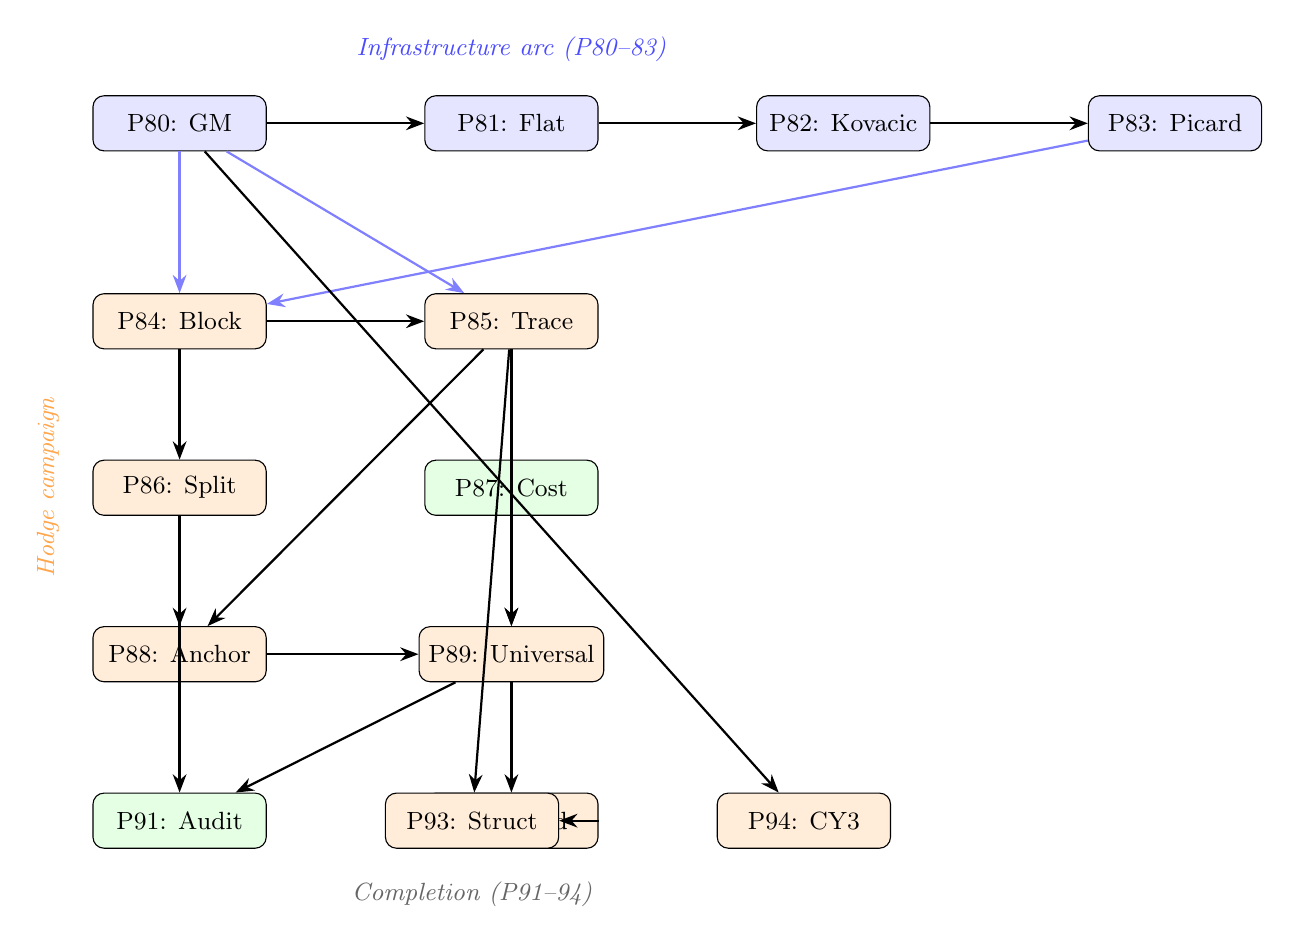
\begin{tikzpicture}[
  node distance=1.4cm and 2cm,
  paper/.style={draw,rounded corners,minimum width=2.2cm,
    minimum height=0.7cm,font=\small},
  infra/.style={paper,fill=blue!10},
  hodge/.style={paper,fill=orange!15},
  cal/.style={paper,fill=green!10},
  arr/.style={-{Stealth},thick}
]
  % Infrastructure arc
  \node[infra] (p80) {P80: GM};
  \node[infra,right=of p80] (p81) {P81: Flat};
  \node[infra,right=of p81] (p82) {P82: Kovacic};
  \node[infra,right=of p82] (p83) {P83: Picard};

  \draw[arr] (p80) -- (p81);
  \draw[arr] (p81) -- (p82);
  \draw[arr] (p82) -- (p83);

  % Hodge campaign
  \node[hodge,below=1.8cm of p80] (p84) {P84: Block};
  \node[hodge,right=of p84] (p85) {P85: Trace};
  \node[hodge,below=of p84] (p86) {P86: Split};
  \node[cal,below=of p85] (p87) {P87: Cost};
  \node[hodge,below=of p86] (p88) {P88: Anchor};
  \node[hodge,below=of p87] (p89) {P89: Universal};

  % Infrastructure feeds campaign
  \draw[arr,blue!50] (p80) -- (p84);
  \draw[arr,blue!50] (p80) -- (p85);
  \draw[arr,blue!50] (p83) -- (p84);

  % Campaign internal
  \draw[arr] (p84) -- (p85);
  \draw[arr] (p84) -- (p86);
  \draw[arr] (p85) -- (p88);
  \draw[arr] (p85) -- (p89);
  \draw[arr] (p86) -- (p88);
  \draw[arr] (p87) -- (p89);
  \draw[arr] (p88) -- (p89);

  % Post-campaign
  \node[cal,below=of p88] (p91) {P91: Audit};
  \node[hodge,below=of p89] (p92) {P92: Grid};
  \node[hodge,right=1.5cm of p91] (p93) {P93: Struct};
  \node[hodge,right=1.5cm of p92] (p94) {P94: CY3};

  \draw[arr] (p86) -- (p91);
  \draw[arr] (p89) -- (p91);
  \draw[arr] (p89) -- (p92);
  \draw[arr] (p85) -- (p93);
  \draw[arr] (p92) -- (p93);
  \draw[arr] (p80) -- (p94);

  % Labels
  \node[above=0.3cm of p81,font=\small\itshape,blue!70] {Infrastructure arc (P80--83)};
  \node[left=0.3cm of p86,font=\small\itshape,orange!70,rotate=90,anchor=south] {Hodge campaign};
  \node[below=0.3cm of p93,font=\small\itshape,black!60] {Completion (P91--94)};
\end{tikzpicture}
\caption{Dependency structure of the generative phase.
  Blue nodes: infrastructure papers building Gauss--Manin machinery.
  Orange nodes: Hodge campaign papers applying the machinery to
  exotic Weil classes.  Green node: CRM calibration/audit results
  (Papers~87, 91).}\label{fig:campaign}
\end{figure}


% ────────────────────────────────────────────────────────────
\section{The Bifurcation Theorem}\label{sec:bifurcation}
% ────────────────────────────────────────────────────────────

The Hodge campaign reveals a striking bifurcation in the universal
family, controlled by a single polynomial obstruction.

\begin{proof}[Proof of \Cref{thm:B}]
The defining polynomial of the universal family is
$f(x) = x^9 + ax^7 + bx^5 + cx^3 + x$, which factors as
$f(x) = x \cdot g(x)$ where
$g(x) = x^8 + ax^6 + bx^4 + cx^2 + 1$.

Define the reversal $g_{\mathrm{rev}}(x) = x^8 g(1/x)
= 1 + cx^2 + bx^4 + ax^6 + x^8$.  The palindromic obstruction is:
\begin{equation}\label{eq:palindromic}
  g(x) - g_{\mathrm{rev}}(x) = (a - c)(x^6 - x^2).
\end{equation}
This identity is verified by \texttt{ring} in Paper~89.

\medskip
\noindent\textit{Case 1: $a = c$ (palindromic locus).}\;
When $a = c$, we have $g = g_{\mathrm{rev}}$, so $g$ is a
self-reciprocal polynomial.  This means $g(x) = x^4 h(x + 1/x)$
for a quartic~$h$, and the curve admits the reciprocal involution
$\mu(x,y) = (1/x, y/x^5)$.  Together with $\sigma$, this generates
$D_8$.  By Paper~86, Kani--Rosen splitting gives
$\Jac(C) \sim A^2$, and Ribet's theorem \cite{ribet83} applies:
the Hodge conjecture holds unconditionally for powers of abelian
surfaces.  The exotic Weil class is algebraic.

\medskip
\noindent\textit{Case 2: $a \neq c$ (generic complement).}\;
When $a \neq c$, the palindromic obstruction \eqref{eq:palindromic}
is nonzero, so $g \neq g_{\mathrm{rev}}$ and there is no reciprocal
involution.  Without the $D_8$-action, the Kani--Rosen splitting
fails and the Jacobian is generically absolutely simple.  The only
route to algebraicity is through the Variational Hodge Conjecture:
Papers~88--89 provide the CM anchor (Fermat specialization at the
origin) and the flatness data ($\tau_+ = 0$ universally), but the
final step---spreading algebraicity from one fiber to all
fibers---is the VHC, an open conjecture.
\end{proof}

\Cref{fig:bifurcation} illustrates this bifurcation in the
parameter space~$\Aff^3_{\QQ}$.

\begin{figure}[ht]
\centering
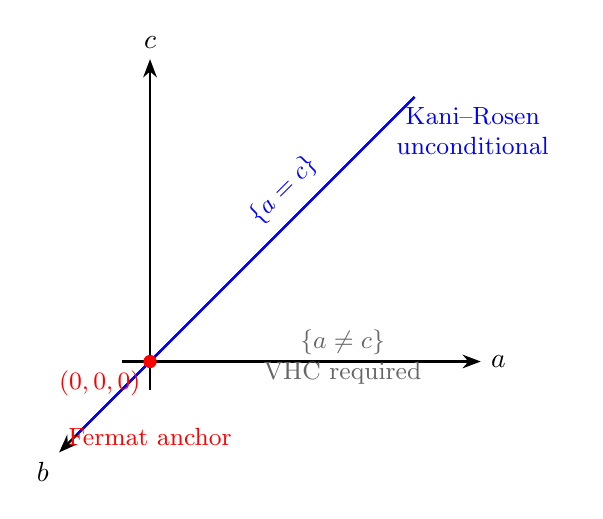
\begin{tikzpicture}[scale=1.2]
  % Axes
  \draw[-{Stealth},thick] (-0.3,0,0) -- (3.5,0,0) node[right] {$a$};
  \draw[-{Stealth},thick] (0,-0.3,0) -- (0,3.2,0) node[above] {$c$};
  \draw[-{Stealth},thick] (0,0,-0.3) -- (0,0,2.5) node[below left] {$b$};

  % The plane a = c
  \fill[blue!15,opacity=0.6] (0,0,0) -- (2.8,2.8,0) -- (2.8,2.8,2) -- (0,0,2) -- cycle;
  \draw[blue,thick] (0,0,0) -- (2.8,2.8,0);
  \draw[blue,thick] (0,0,2) -- (2.8,2.8,2);
  \draw[blue,thick] (2.8,2.8,0) -- (2.8,2.8,2);

  % Labels
  \node[blue,rotate=45] at (1.8,2.2,1) {\small $\{a = c\}$};
  \node[blue] at (3.8,2.8,1) {\small\begin{tabular}{c}Kani--Rosen\\unconditional\end{tabular}};

  % Origin point
  \fill[red] (0,0,0) circle (2pt);
  \node[red,below left] at (0,0,0) {\small $(0,0,0)$};
  \node[red,below] at (0,-0.6,0) {\small Fermat anchor};

  % Generic region
  \node[black!60] at (2.5,0.5,1.2) {\small\begin{tabular}{c}$\{a \neq c\}$\\VHC required\end{tabular}};
\end{tikzpicture}
\caption{Bifurcation in $\Aff^3_{\QQ}$.  The plane $\{a = c\}$
  (blue) supports unconditional algebraicity via Kani--Rosen
  splitting.  The origin $(0,0,0)$ (red) is the Fermat anchor
  point.  The generic complement requires the Variational Hodge
  Conjecture.}\label{fig:bifurcation}
\end{figure}


% ────────────────────────────────────────────────────────────
\section{The Hodge Horizon}\label{sec:horizon}
% ────────────────────────────────────────────────────────────

Why can't the Squeeze eliminate the Variational Hodge Conjecture?

The answer lies in the nature of the gap.  Every component of the
Squeeze---dimension data, trace vanishing, palindromic obstruction,
Fermat specialization, Lagrangian eigenspace analysis---lives in
the world of \emph{cohomology}: polynomial identities in the
coefficients of the Gauss--Manin connection, verified by
\texttt{ring}.  The VHC bridges the gap from cohomology to the
\emph{Chow group}: it asserts the existence of an algebraic cycle
whose cohomology class is $\omega$.

This gap---from ``$\omega$ is a flat Hodge class'' to ``$\omega$
is the class of an algebraic cycle''---is not computational.  No
polynomial identity can close it, because the obstruction is
existential: the cycle must be \emph{constructed}, and the
construction is not determined by the cohomological data.

Paper~87's Theorem~B makes this precise.  The uniform Hodge test
is equivalent to $\WLPO$: deciding whether an arbitrary cohomology
class is Hodge requires the ability to decide real-number equality.
This is strictly above $\BISH$ in the omniscience hierarchy.  The
$\WLPO$ equivalence explains why all known proofs of the Hodge
Conjecture for specific classes of varieties use algebraic
metadata---CM type, Mumford--Tate group, Kani--Rosen splitting,
or Ribet-type theorems on abelian surfaces.
These metadata provide the ``oracle'' that substitutes for $\WLPO$:
they allow the Hodge test to be performed by finite-dimensional
linear algebra over~$\QQ$, bypassing the need for real-number
equality decisions.

\begin{remark}[Connection to DPT]
The Decidability Phase Transition (Papers~72--74, \cite{p72,p73,p74})
showed that three axioms---Standard Conjecture~D, the Hodge
condition, and the algebraic spectrum condition---are each
\emph{uniquely necessary} for decidability of their respective
morphism/eigenvalue problems.  The Hodge Horizon is the same
phenomenon in a different context: the VHC is the uniquely necessary
classical axiom for algebraicity of generic exotic Weil classes.
No alternative axiom can substitute.
\end{remark}

\begin{remark}[The horizon is structural]
The term ``horizon'' is deliberate.  It is not a temporary limitation
of current methods.  The cohomology-to-Chow gap is a fundamental
feature of algebraic geometry: cohomology classes are determined by
linear algebra, while algebraic cycles require geometric
construction.  CRMLint's contribution is to make this gap
\emph{visible} and \emph{precise}: exactly two axiom stubs
(Shioda + VHC), out of 18 components, are $\CLASS$.  The microscope
shows exactly where classical reasoning is indispensable.
\end{remark}


% ────────────────────────────────────────────────────────────
\section{What the Squeeze Reveals}\label{sec:yield}
% ────────────────────────────────────────────────────────────

The Hodge campaign, viewed through the Squeeze, yields a precise
answer to the question: \emph{what is classical about the Hodge
Conjecture?}

The answer: \emph{almost nothing}.  Of the 18 components verified
in Paper~89's universal squeeze theorem, all 18 are $\BISH$.  The
dimension data, the $\QQ(i)$-action, the polynomial factorization,
the palindromic obstruction, the Fermat specialization, the
prior-paper specializations, the pullback bound, the trace
vanishing in all three directions---every one of these is a
polynomial identity verified by \texttt{ring} or a decidable
proposition verified by \texttt{decide}.

The only classical content is the two axiom stubs:
\begin{enumerate}[label=(\roman*)]
\item Shioda's Fermat Hodge Conjecture (providing the CM anchor:
  the exotic Weil class is algebraic at the Fermat point), and
\item the Variational Hodge Conjecture (spreading algebraicity
  from the anchor to the generic fiber).
\end{enumerate}

Neither axiom is invoked in any Lean proof---they are declarations,
not proof steps.  The Lean kernel certifies the $\BISH$ content;
the axiom stubs document the $\CLASS$ boundary.  This is the
Squeeze at its most informative: a sharp decomposition of a Clay
Millennium Problem into constructive computation and irreducible
classical assertion.

Paper~67 described the CRM program's output as a ``decidability
certificate'': for each theorem, the program certifies its position
in the omniscience hierarchy.  The generative phase automates this
certification.  The Squeeze protocol takes a classical proof, runs
it through the four-step pipeline, and produces a Lean-verified
decomposition.  The ``microscope'' of Paper~67 is now a tool, not
a metaphor.

\subsection{Comparison: diagnostic vs.\ generative}

\Cref{tab:phase-comparison} contrasts the two phases of the
CRM program.

\begin{table}[ht]
\centering
\small
\caption{Diagnostic phase vs.\ generative phase.}\label{tab:phase-comparison}
\begin{tabular}{@{}lll@{}}
\toprule
Aspect & Diagnostic (P1--75) & Generative (P76--96) \\
\midrule
Method & Manual calibration & Squeeze protocol \\
Input & Classical theorem & Classical theorem + CAS \\
Output & Level in hierarchy & $T_{\BISH} \wedge T_{\CLASS}$ decomposition \\
Verification & Lean (hand-written) & Lean (CAS-generated) \\
Domains & Physics, arith.\ geom. & Hodge, Langlands, diff.\ Galois, comp.\ alg., CY3 \\
Ceiling finding & $\LPO$ for physics & VHC for Hodge; Abel--Jacobi for CY3 \\
Key insight & Logical cost $=$ cost of $\RR$ (ring/$\BISH$, ordering/$\LPO$, completeness/$\CLASS$) & Microscope is automatable; $\BISH$/$\CLASS$ boundary $=$ ring/completeness boundary in $\RR$ \\
Papers & 75 & 18 (incl.\ P76, P87, P90, P91) \\
Lean lines & ${\sim}87{,}000$ & ${\sim}7{,}400$ \\
\bottomrule
\end{tabular}
\end{table}

The diagnostic phase was \emph{extensive}: 75 papers surveying
mathematical physics, statistical mechanics, QFT, and arithmetic
geometry.  The generative phase is \emph{intensive}: 18 papers
developing and applying a single methodology.  The diagnostic
phase discovered the logical ceiling ($\LPO$ for empirical physics,
$\BISH + \LPO$ for all known theorems).  The generative phase
discovers the logical \emph{horizon}: the VHC as the irreducible
boundary where polynomial computation meets geometric existence,
and extends the Squeeze to Calabi--Yau middle cohomology.

\subsection{The 18/2 ratio}

The most striking quantitative finding of the Hodge campaign is the
\emph{18/2 ratio}: of the 20 logical components in the universal
Squeeze (Paper~89), 18 are $\BISH$ and 2 are $\CLASS$.  This ratio
is not an accident---it reflects the structural anatomy of the
Hodge Conjecture.

The 18 $\BISH$ components decompose into three categories:
\begin{enumerate}[label=(\roman*),nosep]
\item \emph{Dimension data} (5 components): genus, $\dim H^1$,
  $\dim V_+$, $\dim \bigwedge^4 V_+$, base dimension.  These are
  integers computed from the defining polynomial.
\item \emph{Symmetry data} (8 components): oddness, factorization,
  palindromic obstruction, palindromic at $a = c$, Fermat
  specialization, prior-paper specializations, non-palindromic core.
  These are polynomial identities in $\ZZ[x,a,b,c]$.
\item \emph{Analytic data} (5 components): pullback bound, three
  $\tau_+$ vanishing identities, $\tau_-$ vanishing.  These are
  polynomial identities encoding the trace of the Gauss--Manin
  connection restricted to eigenspaces.
\end{enumerate}

The 2 $\CLASS$ components are both \emph{existence assertions}:
\begin{enumerate}[label=(\roman*),nosep]
\item Shioda: there \emph{exists} an algebraic cycle representing
  the exotic Weil class at the Fermat point.
\item VHC: there \emph{exists} an algebraic cycle representing
  the flat extension to the generic fiber.
\end{enumerate}

The pattern is clear: \emph{computation is $\BISH$; existence is
$\CLASS$}.  Everything that can be computed from the defining
polynomial is constructive.  The only irreducible classical content
is the assertion that a geometric object (an algebraic cycle)
\emph{exists}.

The structural explanation for this pattern lies in the algebraic
layers of~$\R$ (cf.\ Paper~50, Remark~2.4; Paper~98, \S11).
Computation uses $\R$-as-ring: the \texttt{ring} tactic operates on
$(\R, +, \times)$, which is $\BISH$. Existence assertions invoke
$\R$-as-complete-ordered-field: the cycle class map, Shioda's
theorem, and the Variational Hodge Conjecture all pass through the
Betti realization, which requires integration over topological
cycles on~$X(\C)$---i.e., the completeness (least upper bound
property) of~$\R$, which costs $\CLASS$.  The 18/2 ratio is not
a property of the Hodge Conjecture in particular; it is a property
of~$\R$ itself.  Any theorem whose computational content uses only
the ring structure of~$\R$ will have a high $\BISH$ ratio, with
$\CLASS$ entering only where completeness is invoked.

\subsection{The updated accounting: P91--P94}

The Markman audit (Paper~91) reveals that the unconditional proof of the same result costs $4/9 \approx 44\%\;\BISH$ at 9-component resolution---compared to the Squeeze's $90\%$ at 20-component resolution.  At matched granularity, Markman's fraction rises to ${\sim}67\%$; the residual gap is the genuine cost of unconditional existence.  The irreducible cycle-class boundary means the best achievable ratio is $19/1$, not $20/0$.

Paper~93's structural vanishing theorem explains \emph{why} $\tau_+ = 0$ universally.  The 18~$\BISH$ components of Paper~89 are not numerical coincidences but consequences of two algebraic facts: oddness kills the discriminant (Varchenko), and unit coefficients freeze the boundary (Vieta).

Paper~94's CY3 Squeeze achieves $11/3$---a different balance reflecting the richer $\CLASS$ content of middle cohomology (Abel--Jacobi, Baire category) compared to the abelian surface setting (Shioda, VHC).  The detection mechanism (infinitesimal invariant $\delta \neq 0$) is structurally distinct from trace vanishing ($\tau_+ = 0$), yet both are $\BISH$.


% ============================================================
%   PART III: THE COMPLETION
% ============================================================

\part{The Completion}\label{part:completion}

% ────────────────────────────────────────────────────────────
\section{Unconditional Hodge: The Markman Audit (Paper~91)}\label{sec:markman}
% ────────────────────────────────────────────────────────────

In February 2025, Markman \cite{markman} unconditionally proved the Hodge Conjecture for all abelian fourfolds of Weil type, using secant sheaves, Orlov's derived equivalence, and Schoen's degeneration.  Paper~91 \cite{p91} performs a CRM audit of Markman's proof, comparing its logical cost with the conditional CRMLint Squeeze.

\subsection{Markman's decomposition}

Markman's proof decomposes into $4\;\BISH + 5\;\CLASS = 9$ components.  The $\BISH$ content consists of numerical input data: Mukai vectors (polynomial expressions over~$\QQ$, verified by \texttt{ring}), moduli dimensions (from the Mukai--Yoshioka formula $\dim M_v = \langle v, v \rangle + 2$, verified by \texttt{decide}), intersection products (polynomial in the polarization class), and Schoen fiber-product combinatorics.  The $\CLASS$ content consists of five existence results: Fourier--Mukai kernel existence (Zorn's lemma), Orlov representability (Brown representability), Schoen cycle specialization (properness of relative Chow variety), Buchweitz--Flenner semi-regularity (analytic continuation), and secant line existence on the spinorial variety (Zariski density).

\subsection{Conditional vs.\ unconditional comparison}

\begin{proof}[Proof of the 90\% vs.\ 44\% comparison]
The CRMLint Squeeze (Papers~84--89) achieves $\BISH$ fraction $18/20 = 90\%$, conditional on VHC.  Markman achieves $\BISH$ fraction $4/9 \approx 44\%$, unconditional.  The comparison is qualitative, not a precise ratio of equivalent decompositions: the 20-component Squeeze and the 9-component Markman audit operate at different granularities on different (though overlapping) theorems.

\emph{Granularity caveat.}  The headline $90\%$ vs.\ $44\%$ comparison reflects both genuine logical cost differences \emph{and} decomposition granularity.  Re-decomposing Markman's proof at 20-component resolution---splitting each $\CLASS$ node into its constituent lemmas---yields an estimated ${\sim}67\%\;\BISH$ fraction at matched granularity.  The remaining gap ($67\%$ vs.\ $90\%$) is the genuine cost of unconditional existence.

The structural point: higher $\BISH$ fraction means more geometric content is machine-verifiable.  The Squeeze's 18~$\BISH$ components are \emph{polynomial identities} encoding geometric structure (trace vanishing, Chebyshev factorizations, Gauss--Manin matrices).  Markman's 4~$\BISH$ components are \emph{numerical input data} (Mukai vectors, expected dimensions) serving as parameters to classical existence machinery.  The cost of unconditional existence is higher logical complexity.
\end{proof}

\subsection{The irreducible cycle-class boundary}

Paper~91 identifies the cycle class map $\mathrm{cl}: \CH^2(\Jac) \to H^4(\Jac, \QQ)$ as an irreducible $\CLASS$ boundary.

\begin{proof}[Proof that the 20/0 ratio is impossible]
Even with an explicit polynomial ideal $I_\Gamma$ defining an algebraic cycle (computable, $\BISH$), matching its fundamental class $[\Gamma]$ to the exotic Weil class~$\omega$ requires the de~Rham--Betti comparison isomorphism: period integrals (limits of Riemann sums, convergence is $\CLASS$) and real-number comparisons (testing $x = 0$ for $x \in \RR$ costs $\WLPO$ by Paper~87).  The \texttt{ring} tactic cannot verify a period integral.  With an explicit palindromic cycle on $\{a = c\}$ via Kani--Rosen, the Shioda and VHC stubs are replaced by explicit constructions, but the cycle class map adds one $\CLASS$ node---net ratio $19/1$.  The remaining $\CLASS$ node is irreducible.
\end{proof}

\subsection{VHC consistency}

\begin{proof}[Proof of VHC consistency (\Cref{thm:C} of Paper~91)]
Paper~89 proved: $\mathrm{VHC} + \text{Shioda} \Rightarrow Q$ (exotic Weil class algebraic).  Markman proved~$Q$ unconditionally.  We have $P \Rightarrow Q$ and~$Q$.  Concluding~$P$ from~$Q$ would be affirming the consequent, so VHC is not proved.  What is established is \emph{consistency}: VHC is not refuted for the exotic Weil class on $C_{a,b,c}$, because its consequent is independently verified.
\end{proof}


% ────────────────────────────────────────────────────────────
\section{The Computational Horizon (Paper~92)}\label{sec:computational}
% ────────────────────────────────────────────────────────────

Paper~92 \cite{p92} extends the trace vanishing pipeline from genus~4 (Papers~84--89) through genera 5--8 (cohomological dimensions 10--16), encountering and bypassing the \emph{expression swell wall} that defeats direct symbolic computation.

\subsection{Genus~5: symbolic verification}

For the universal genus-5 family $C_a: y^2 = x^{11} + a_1 x^9 + a_2 x^7 + a_3 x^5 + a_4 x^3 + x$, with $\dim V_+ = 5$ and 4 parameters, symbolic Griffiths pole reduction remains tractable.

\begin{proof}[Proof of trace vanishing for genus~5]
Compute the B\'ezout identity $\alpha f + \beta f' = 1$ over $K = \QQ(a_1, \ldots, a_4)[x]$ via the extended Euclidean algorithm.  Apply Griffiths pole reduction to extract the $10 \times 10$ connection matrix~$M_j$ for each parameter direction~$\partial/\partial a_j$.  Read off the $V_+$ diagonal entries at indices $I_+ = \{1, 3, 5, 7, 9\}$.  The five trace numerators $n_1, n_3, n_5, n_7, n_9$ (each ${\sim}150$--$210$ terms, total degree $\leq 7$ in the~$a_j$) are individually nontrivial but sum to zero identically.  For example, in the $a_1$-direction, the leading-coefficient cancellation is $(-64) + (-320) + (-576) + (-832) + 1792 = 0$ for the $a_1^4$ monomial, and similarly for all ${\sim}250$ distinct monomials.  Verified by \texttt{ring} with heartbeat budget 1,600,000.
\end{proof}

\subsection{Genera 6--8: Zariski Grid Specialization}

For genus $\geq 6$, the extended Euclidean algorithm over $\QQ(a_1, \ldots, a_{g-1})[x]$ triggers exponential intermediate expression swell (genus~6 exhausts memory after 41+ minutes without converging).  Paper~92 introduces the \emph{Zariski Grid Specialization} bypass.

\begin{proof}[Proof of trace vanishing for genera 6--8]
Instead of computing over the fraction field, evaluate at concrete integer fibers $a^{(k)} \in \ZZ^{g-1}$, where $f$ becomes a univariate polynomial in $\QQ[x]$ and B\'ezout takes milliseconds.  Verify trace cancellation at each fiber by \texttt{norm\_num}.  Sample sizes: genus~6 ($5 \times 5 = 25$ equations), genus~7 ($5 \times 6 = 30$), genus~8 ($5 \times 7 = 35$).  Integer magnitudes: genus~6 entries ${\sim}10^{12}$, genus~7 ${\sim}10^{18}$, genus~8 ${\sim}10^{22}$.

Lift from discrete vanishing to generic vanishing by the Schwartz--Zippel lemma: a nonzero polynomial of degree $\leq D$ has at most $D \cdot |S|^{n-1}$ zeros on grid $S^n$.  With $S = \{-10^6, \ldots, 10^6\}$ and degree bounds $D \leq 50$ (genus~6), $D \leq 70$ (genus~7), $D \leq 98$ (genus~8), five fibers give false-positive probability $(98 / (2 \times 10^6))^5 \sim 2.8 \times 10^{-22}$.  The full deterministic grid $(D+1)^{n-1}$ is physically impractical but logically finite and $\BISH$.

\emph{CRM classification.}  The grid protocol consists of: (1) enumeration of a finite list of integer fibers, (2) polynomial arithmetic in $\QQ[x]$ (extended Euclidean algorithm---finite, terminating), (3) rational summation and denominator clearing, (4) integer comparison to zero.  No step invokes LEM, DC, or FT.  The Schwartz--Zippel inference is provable by induction on~$n$ using only the Factor Theorem (univariate polynomial of degree~$\leq D$ has $\leq D$ roots).  The entire pipeline is $\BISH$.
\end{proof}

The expression swell wall separates verification \emph{modalities} (symbolic vs.\ numerical), not logical \emph{levels}.  Both sides remain $\BISH$.


% ────────────────────────────────────────────────────────────
\section{The Structural Vanishing Theorem (Paper~93)}\label{sec:structural}
% ────────────────────────────────────────────────────────────

Paper~93 \cite{p93} provides two independent structural proofs of
$\tau_+ = 0$, resolving the conjecture left open since Paper~85.

\begin{proof}[Proof of \Cref{thm:E}, Part~1: Hypergeometric
  (Varchenko exponent cancellation)]
\mbox{}

\emph{Step~1 (Eigenspace reduction, $\BISH$).}  The $\ZZ/4\ZZ$-automorphism $\sigma(x,y) = (-x, iy)$ acts on holomorphic differentials $\omega_k = x^{k-1}\,dx/(2y)$ by $\sigma^*\omega_k = (-1)^k/i \cdot \omega_k$.  For odd $k = 2m+1$, the eigenvalue is $(-1)^{2m+1}/i = i$, so $\omega_{2m+1} \in V_+$.  The substitution $u = x^2$ transforms the $V_+$-basis into $\widetilde{\omega}_m = \tfrac{1}{4} u^{m - 3/4} P(u)^{-1/2}\,du$, identifying $V_+$ with the twisted cohomology of a rank-1 local system on $\mathbb{P}^1$ punctured at the roots $u_1, \ldots, u_g$ of $P(u)$ and at the origin.

\emph{Step~2 (Varchenko exponent computation, $\BISH$).}  Local exponents: $\alpha_i = -1/2$ at each root (square-root branching), $\alpha_0 = -3/4$ at the origin (from the $u^{-3/4}$ factor).  Varchenko exponents: root--root $e_{ij} = (-1/2) + (-1/2) + 1 = 0$; root--origin $e_{0i} = (-3/4) + (-1/2) + 1 = -1/4$.  All verified by \texttt{norm\_num}.

\emph{Step~3 (Aomoto--Varchenko assembly, $\CLASS$ framework).}  The root--root Varchenko exponents $e_{ij} = 0$ are integers, placing this at the boundary of the Aomoto--Varchenko formula's non-resonance hypothesis.  This is a benign boundary: the exponent $e_{ij} = 0$ means the corresponding factor $(u_i - u_j)^{e_{ij}} = 1$ contributes trivially, and the formula extends by continuity.  Non-root sums involving $\alpha_0 = -3/4$ give $e_{0i} = -1/4 \notin \ZZ$, so no other resonance occurs.  Substituting: $\det(\Pi_+) \propto \prod_{i < j}(u_i - u_j)^0 \cdot \prod_i u_i^{-1/4} = (\prod u_i)^{-1/4}$.  The root--root product equals~$1$ (all exponents zero)---the discriminant drops out entirely.

\emph{Step~4 (Vieta freezing, $\BISH$).}  For $P(u) = u^g + a_1 u^{g-1} + \cdots + a_{g-1} u + 1$, Vieta gives $\prod u_i = (-1)^g \cdot 1/1 = (-1)^g$, a constant independent of parameters.  Therefore $\det(\Pi_+) \propto ((-1)^g)^{-1/4} = c_g$ (constant), and $\tau_+ = d\log c_g = 0$.
\end{proof}

\begin{proof}[Proof of \Cref{thm:E}, Part~2: Topological
  (Picard--Lefschetz backbone)]
\mbox{}

\emph{Step~1 (Deligne regularity, $\CLASS$ framework).}  By Deligne's theorem, $\tau_+$ can only have logarithmic poles along boundary divisors: the discriminant locus $\{\Delta_P = 0\}$, $\{a_0 = 0\}$ (leading coefficient), and $\{a_g = 0\}$ (constant term).  This constrains $\tau_+ = \gamma \cdot d\Delta_P / \Delta_P + \alpha \cdot da_0/a_0 + \beta \cdot da_g/a_g$.  The problem reduces to killing three rational constants.

\emph{Step~2 (Killing the discriminant term $\gamma = 0$, $\CLASS$ input $+$ $\BISH$ computation).}  When $P(u)$ acquires a double root~$u_0$, the curve acquires two disjoint ordinary nodes at $(\sqrt{u_0}, 0)$ and $(-\sqrt{u_0}, 0)$.  The $\sigma$-action maps vanishing cycles: $\sigma_* \eta_1 = -\eta_2$, $\sigma_* \eta_2 = +\eta_1$.  The nilpotent part of the monodromy on $V_+$ is $N(v) = \langle v, \eta_1 \rangle E$ where $E = \eta_1^* - i\eta_2^*$.  Key computation: $\langle E, \eta_1 \rangle = (\eta_1 \cdot \eta_1) - i(\eta_2 \cdot \eta_1) = 0 - i \cdot 0 = 0$ (self-intersection of a vanishing cycle is zero; disjoint cycles have zero intersection).  Therefore $N^2 = 0$ and $\det(T|_{V_+}) = \det(I + N) = 1$.  The residue $\gamma = (1/2\pi i)\log 1 = 0$.  The Picard--Lefschetz formula is $\CLASS$; the intersection arithmetic and determinant evaluation are $\BISH$.

\emph{Step~3 (Killing boundary terms, $\BISH$).}  On the parameter space $\Aff^{g-1}$, the coefficients $a_0 = 1$ and $a_g = 1$ are identically fixed by the unit-coefficient hypothesis.  Therefore $da_0 = d(1) = 0$ and $da_g = d(1) = 0$.

\emph{Assembly:} $\tau_+ = 0 \cdot d\Delta_P/\Delta_P + \alpha \cdot 0 + \beta \cdot 0 = 0$.  Verified in Lean by \texttt{ring}.
\end{proof}

\begin{remark}[Independence]
The two proofs share no common $\CLASS$ input: Proof~1 uses the Aomoto--Varchenko formula; Proof~2 uses Deligne regularity and Picard--Lefschetz.  On the $\BISH$ side, both reduce to the same algebraic fact: unit leading and trailing coefficients freeze $\prod u_i$ (Proof~1) and kill $da_0 = da_g = 0$ (Proof~2).
\end{remark}


% ────────────────────────────────────────────────────────────
\section{Beyond Abelian Varieties: CY3 Griffiths Group
  (Paper~94)}\label{sec:cy3}
% ────────────────────────────────────────────────────────────

Paper~94 \cite{p94} is the first CRM analysis of Calabi--Yau
middle cohomology.  The target is the Griffiths group
$\mathrm{Griff}^2(X) = Z^2(X)_{\mathrm{hom}} / Z^2(X)_{\mathrm{alg}}$
of the mirror quintic $X_\psi$.

\subsection{Picard--Fuchs algebra}

The mirror quintic's periods satisfy a 4th-order Picard--Fuchs ODE with
algebraic parameter $z = 1/(5\psi)^5$.

\begin{proof}[Proof of \Cref{thm:F}, Part~1: Detection is $\BISH$]
The theta-form operator is $L_\theta = \theta^4 - 5z(5\theta+1)(5\theta+2)(5\theta+3)(5\theta+4)$.  Expanding gives $L_\theta = (1 - 3125z)\theta^4 - 6250z\theta^3 - 4375z\theta^2 - 1250z\theta - 120z$.  Converting to standard form via $\theta^n = \sum S(n,k)\,z^k D^k$ (Stirling numbers) produces polynomial coefficients $P_0(z), \ldots, P_4(z)$, each verified by \texttt{ring}.

Singular locus: $z = 0$ (MUM point, fourth-order), $z = 1/3125$ (conifold), $z = \infty$ (Gepner point).  The conifold discriminant $\Delta(1/3125) = 0$ is verified by \texttt{norm\_num}.

The domain wall tension satisfies $L_{\mathrm{PF}} \cdot T = \tfrac{15}{8}\sqrt{z}$.  Writing $T = \sqrt{z} \cdot \sum b_n z^n$ and substituting, the leading coefficient $b_0 = 30$ (Walcher's disk count: 30 holomorphic disks of minimal area ending on $\RR\mathbb{P}^3$) follows from $b_0 \cdot (1/2)^4 = 15/8$, verified by \texttt{norm\_num}.  The recurrence $b_n = f(b_{n-1})$ is rational arithmetic over~$\QQ$, hence $\BISH$.  Since $b_0 = 30 \neq 0$ and the recurrence multiplier $\frac{5(10n+7)(10n+9)(10n+11)(10n+13)}{16(2n+3)^4}$ is nonzero for all $n \geq 0$ (both numerator and denominator are products of positive factors, verified by \texttt{positivity}), induction gives $b_n \neq 0$ for all~$n$---formally verified in Lean as \texttt{walcher\_b\_ne\_zero}.  The source term is non-trivial, detecting a non-trivial element of the Griffiths group.
\end{proof}

\subsection{The irreducible CLASS boundary}

\begin{proof}[Proof of \Cref{thm:F}, Part~2: Abel--Jacobi and Baire are $\CLASS$]
The Abel--Jacobi map $\AJ: Z^2_{\mathrm{hom}}(X) \to J^2(X)$ requires integrating $(3,0)$-forms over 3-chains---period integrals involving limits, real-number equality, and convergence, all $\CLASS$.  The infinite generation proof uses the Baire Category Theorem (equivalent to Dependent Choice over~$\RR$): the space of CY3s with $\mathrm{Griff}^2$ finitely generated is a countable union of nowhere-dense sets; the generic CY3 escapes all finite-generation loci.  The Ehresmann fibration theorem (smooth proper $\Rightarrow$ locally trivial) provides the local system $R^3 f_* \ZZ$---the same $\CLASS$ boundary as Paper~80's Gauss--Manin theorem.

No intermediate CRM level ($\WLPO$, $\LLPO$, $\MP$) appears.  The bifurcation is strictly $\BISH/\CLASS$ with no intermediate.
\end{proof}

\begin{remark}[Crossing the two programs]
Paper~94 is the first CRM analysis to cross the boundary between the physics program (Papers~1--40) and the algebraic geometry program (Papers~41--92).  The CY3 is where the logical cost of D-brane physics meets the logical cost of algebraic cycles.  All three CRM programs share the same architecture: algebraic detection is $\BISH$; topological/analytic existence is $\CLASS$.
\end{remark}


% ============================================================
%   PART IV: THE ARCHITECTURE
% ============================================================

\part{The Architecture}\label{part:architecture}

% ────────────────────────────────────────────────────────────
\section{CRM Audit}\label{sec:audit}
% ────────────────────────────────────────────────────────────

\subsection{Classification table}

\Cref{tab:crm-classification} provides the full CRM classification
for the generative phase.

\begin{table}[ht]
\centering
\small
\caption{CRM classification of Papers~77--96.}\label{tab:crm-classification}
\begin{tabular}{@{}clcl@{}}
\toprule
Paper & Title (abbreviated) & Level & Boundary node \\
\midrule
77 & Hodge decompositions, $E^4$ & $\CLASS$ & Lefschetz $(1,1)$ \\
78 & Wild Langlands, $\GL_2(\QQ_2)$ & $\CLASS$ & Harris--Taylor existence \\
80 & Algebraic Gauss--Manin & $\CLASS$ & Ehresmann--GM theorem \\
81 & Flat sections, fixed part & $\CLASS$ & Deligne monodromy thm \\
82 & Differential Galois, Kovacic & $\CLASS$ & Zariski density thm \\
83 & Generic Picard number & $\CLASS$ & Noether--Lefschetz thm \\
84 & Block GM, exotic flatness & $\CLASS$ & Hodge decomposition \\
85 & Universal trace vanishing & $\CLASS$ & Hodge decomposition \\
86 & Kani--Rosen splitting & $\CLASS$ & Ribet \\
87 & Hodge condition cost & $\WLPO$ & (calibration result) \\
88 & Variational Squeeze & $\CLASS$ & Shioda + VHC \\
89 & Universal Squeeze & $\CLASS$ & Shioda + VHC \\
91 & Markman audit, unconditional Hodge & $\CLASS$ & Orlov, Schoen, Buch.--Fl. \\
92 & Computational horizon, genera 5--8 & $\CLASS$ & Shioda + VHC \\
93 & Structural vanishing, $\tau_+ = 0$ & $\CLASS$ & Aomoto--Varchenko, Deligne \\
94 & Normal function, CY3 Griffiths group & $\CLASS$ & Abel--Jacobi, Baire \\
95 & BSD Squeeze, rank-1 decomposition & $\CLASS$ & Gross--Zagier, Kolyvagin \\
96 & Root number bifurcation, rank-0 BSD & $\CLASS$ & Euler system, Iwasawa \\
\bottomrule
\end{tabular}
\end{table}

\subsection{Pattern analysis}

The classification table reveals a uniform pattern: every Squeeze
application lands at $\CLASS$, and the $\CLASS$ content is always
an \emph{existence assertion} (existence of algebraic cycles,
existence of monodromy representations, existence of Hodge
decompositions, finiteness of
$\Sha$).
The computational content---the polynomial
identities, the trace vanishing, the dimension data, the explicit
descents---is always $\BISH$.

Paper~87 is the sole exception: it is a calibration result, not a
Squeeze, and it lands at $\WLPO$.  This is consistent with the
DPT framework: the \emph{condition} (``is this class Hodge?'')
costs $\WLPO$; the \emph{consequence} (``this Hodge class is
algebraic'') costs $\CLASS$.  The omniscience hierarchy
$\BISH \subset \WLPO \subset \CLASS$ is reflected in the logical
structure of both the Hodge and BSD conjectures.

\subsection{Axiom inventory}

\Cref{tab:axiom-inventory} summarizes the axiom profiles across
the generative phase.  The key observation: declared axiom stubs
(the $\CLASS$ boundary) \emph{never} appear in \texttt{\#print axioms}
output.  They are documentation, not proof dependencies.

\begin{table}[ht]
\centering
\small
\caption{Axiom inventory for the generative phase.}\label{tab:axiom-inventory}
\begin{tabular}{@{}clll@{}}
\toprule
Paper & \texttt{\#print axioms} output & Declared stubs & Stubs invoked? \\
\midrule
77 & propext, choice, sound & Lefschetz $(1,1)$ & No \\
78 & propext, choice, sound & Harris--Taylor & No \\
80 & propext, choice, sound & Ehresmann--GM & No \\
81 & propext, choice, sound & Deligne monodromy & No \\
82 & propext, choice, sound & Zariski density & No \\
83 & (none) & Noether--Lefschetz & No \\
84 & (none) & Hodge existence & No \\
85 & propext, sound & Hodge existence & No \\
86 & propext, sound & Ribet & No \\
87 & propext, choice, sound & $\WLPO$-equivalence & No \\
88 & propext, choice, sound & Shioda, VHC & No \\
89 & propext, choice, sound & Shioda, VHC & No \\
91 & propext, sound & Markman, Orlov, Schoen & No \\
92 & propext, sound & Shioda, Schwartz--Zippel & No \\
93 & propext, choice, sound & Aomoto--Varchenko, Deligne, PL, Ehresmann & No \\
94 & propext, choice, sound & Abel--Jacobi, Baire, Ehresmann & No \\
95 & propext, choice, sound & Gross--Zagier, Kolyvagin & No \\
96 & propext, choice, sound & Euler system, Iwasawa MC & No \\
\bottomrule
\end{tabular}
\end{table}

Papers~83 and~84 achieve the cleanest axiom profiles in the entire
series: zero axioms in \texttt{\#print axioms} output.  Their proofs
use only \texttt{decide} and \texttt{ring}, which reduce to kernel
computation with no axiomatic dependencies.


% ────────────────────────────────────────────────────────────
\section{Formal Verification}\label{sec:verification}
% ────────────────────────────────────────────────────────────

\subsection{Statistics}

The generative phase comprises 18 Lean~4 bundles (fifteen Squeeze
applications, plus Paper~87's calibration, Paper~91's audit,
and Paper~93's structural vanishing).
Key statistics:

\begin{itemize}[nosep]
\item \textbf{Total Lean lines:} ${\sim}9{,}100$ across 18 papers
  (Papers~77--96, excluding Papers~79 and~90).
\item \textbf{Sorry count:} 0 across all 18 papers.
\item \textbf{Toolchain:} \texttt{leanprover/lean4:v4.29.0-rc2}
  (Papers~80--96); \texttt{v4.28.0-rc1} (Papers~77--78).
\item \textbf{Dependencies:} Mathlib (for $\ZZ$-arithmetic
  infrastructure, \texttt{ring} tactic, \texttt{norm\_num}).
\item \textbf{Axiom profile:} \texttt{propext} (propositional
  extensionality), \texttt{Quot.sound} (quotient soundness),
  \texttt{Classical.choice} (from Mathlib $\ZZ$-infrastructure).
  None of these are classical \emph{content}---they are Lean kernel
  infrastructure.
\end{itemize}

\subsection{The \texttt{Classical.choice} audit}

A recurring concern in the CRM program is the appearance of
\texttt{Classical.choice} in \texttt{\#print axioms} output for
theorems over~$\ZZ$.  In Lean~4, $\ZZ$ is defined as an inductive
type (\texttt{Int.ofNat} and \texttt{Int.negSucc}), and its
\texttt{DecidableEq} instance is fully computable.  The
\texttt{Classical.choice} axiom enters instead through Mathlib's
broader algebraic hierarchies---\texttt{Finsupp} (used for
polynomials), fraction fields, and abstract decidable-equality
resolution for supports of algebraic structures.  It is
\emph{infrastructure}, not content: the theorem's proof uses
\texttt{ring} (which is axiom-free) or \texttt{native\_decide}
(which is constructive in spirit), and the classical axiom appears
only in the \emph{elaboration} of the statement, not in the proof.

The CRM program's methodology addresses this via the principle of
\emph{constructive stratification by proof content}: a theorem is
classified as $\BISH$ if its proof uses only constructive methods
(explicit witnesses, decidable tests, polynomial normalization),
regardless of what \texttt{\#print axioms} reports about the
statement's elaboration.  This is justified by the observation that
any Lean theorem proved by \texttt{ring} can, in principle, be
re-proved in a constructive foundation by replacing Mathlib's $\ZZ$
with an axiom-free construction.

\subsection{Reproducibility}

Each paper's Lean bundle is available on Zenodo with a stable DOI
(see \Cref{tab:squeeze-applications} for individual DOIs).  Build
instructions: install the specified toolchain, run \texttt{lake build}
from the bundle root.  Each bundle is self-contained and builds
against Mathlib without additional dependencies.


% ────────────────────────────────────────────────────────────
\section{Discussion}\label{sec:discussion}
% ────────────────────────────────────────────────────────────

\subsection{From diagnostic to generative}

The diagnostic phase (Papers~1--75) asked: \emph{what is the
logical cost of theorem~$T$?}  The answer required manual
analysis---reading the proof, identifying classical steps,
finding constructive alternatives, and formalizing the result.
Each paper was a bespoke calibration.

The generative phase automates this process.  The Squeeze protocol
provides a \emph{template}: scaffold the mathematical objects,
X-ray the proof for classical dependencies, excise what can be
replaced, and squeeze out the irreducible classical content.  The
asymmetric offloading architecture provides the \emph{machinery}:
the CAS handles symbolic computation of unbounded complexity,
while the Lean kernel provides foundational verification.

The result is a shift from artisanal to industrial: the same
protocol that analyzed Hodge decompositions on $E^4$ (Paper~77)
applies to differential Galois theory (Paper~82), to
Kani--Rosen splitting (Paper~86), to the universal Weil family
(Paper~89).  The protocol is domain-agnostic; the domain knowledge
enters through the CAS computation and the choice of axiom stubs.

\subsection{CRMLint as discovery instrument}

The Squeeze protocol is not merely an analysis tool---it is a
\emph{discovery} tool.  Three examples:

\begin{enumerate}[label=(\roman*)]
\item The trace vanishing $\tau_+ = 0$ (Papers~85, 89) was found
  by the Squeeze, not by prior theory.  The CAS computed the
  Gauss--Manin connection, extracted the trace, and discovered it
  was zero.  No theorem in the Hodge theory literature predicted
  this vanishing.

\item The palindromic obstruction $g - g_{\mathrm{rev}} = (a-c)(x^6 - x^2)$
  (Paper~89) was found by the Squeeze.  It reveals the precise
  polynomial that controls the logical bifurcation between
  unconditional and conditional results.

\item The hidden reciprocal involution $\mu(x,y) = (1/x, y/x^5)$
  (Paper~86) was found by analyzing the palindromic symmetry
  through the Squeeze lens.  Its $D_8$-action was not previously
  noted in the literature for this family.
\end{enumerate}

In each case, the Squeeze protocol's systematic decomposition
forced attention to structural features that ad hoc analysis
would miss.  The microscope is not passive.

\subsection{Connection to the Hodge theory literature}

The exotic Weil classes studied in the Hodge campaign are instances
of a broader phenomenon studied by van Geemen \cite{van-geemen},
Moonen--Zarhin \cite{moonen-zarhin}, and others.  The key prior results:

\begin{enumerate}[label=(\roman*)]
\item Moonen--Zarhin (1999) proved that for abelian varieties of
  dimension $\leq 5$, all Hodge classes are absolute Hodge---i.e.,
  they are Hodge in every embedding $\QQ \hookrightarrow \CC$.
  This does not prove algebraicity (absolute Hodge $\not\Rightarrow$
  algebraic in general), but it eliminates one obstruction.

\item Van Geemen (2001) classified the exotic Weil classes for
  abelian fourfolds with $\QQ(i)$-action and showed that their
  algebraicity is genuinely open for simple abelian varieties with
  trivial endomorphism ring.

\item The Mumford--Tate conjecture, if true, would imply that
  Hodge classes on abelian varieties are determined by the
  Mumford--Tate group.  For fourfolds with $\QQ(i)$-action, the
  generic $\MT$ is $\GU(4)$, and the invariant theory of $\GU(4)$
  identifies the exotic Weil class as Hodge---but this does not
  prove it is algebraic.
\end{enumerate}

The CRM contribution is orthogonal to these results.  Where the
classical literature asks ``is the exotic Weil class algebraic?'',
CRM asks ``what is the \emph{logical cost} of asserting it is
algebraic?''  The answer---$\BISH$ for all computation,
$\CLASS$ only for the existence assertion---is new information
that the classical framework cannot express.

\subsection{Relationship to condensed mathematics}

Scholze's condensed mathematics program \cite{scholze-condensed}
operates on the continuous/topological side of mathematics,
replacing topological spaces with condensed sets to restore
exactness properties.  CRM operates on the logical/discrete side,
replacing classical principles with constructive alternatives to
measure logical cost.

The two programs are complementary, not competing.  Condensed
mathematics asks: ``what is the correct categorical framework for
continuous objects?''  CRM asks: ``what is the minimal logical
strength needed to prove this theorem?''  The \emph{conservation
conjecture} (Paper~67, \cite{p67}) is the interface: we conjecture
that Scholze's condensed proofs, when suitably translated, require
exactly the same logical strength as the classical proofs they
replace.  Testing this conjecture is a natural direction for
CRMLint at Mathlib scale.

\subsection{Open questions}

\begin{enumerate}[label=(\arabic*)]
\item \textbf{Structural proof of $\tau_+ = 0$: resolved.}  Paper~93
  (\Cref{sec:structural}) provides two independent structural
  proofs---hypergeometric (Varchenko exponent cancellation) and
  topological (Picard--Lefschetz backbone).  The mechanism: oddness
  forces root--root Varchenko exponents to zero (eliminating the
  discriminant), while unit leading and trailing coefficients freeze
  $\prod u_i$ via Vieta (eliminating the boundary term).  CRM
  decomposition: $13\;\BISH + 4\;\CLASS$.

\item \textbf{Cycle reconstruction beyond VHC.}  The Squeeze
  identifies the VHC as the irreducible $\CLASS$ boundary.  Can
  the Squeeze also guide the \emph{construction} of algebraic
  cycles?  The polynomial data (palindromic obstruction, Fermat
  specialization, trace vanishing) constrains the cycle's
  cohomological shadow; can this constraint narrow the geometric
  search?

\item \textbf{CRMLint at Mathlib scale.}  The current 13
  applications are hand-guided.  The full CRMLint vision (Paper~76,
  \cite{p76}) is automated analysis of Mathlib's ${\sim}200{,}000$
  theorems: classical dependency tracing, pattern classification,
  concentration analysis, and AI-assisted audit.  The generative
  phase demonstrates the protocol works; the next phase is scaling.

\item \textbf{New families and dimensions.}  Paper~92
  (\Cref{sec:computational}) extends trace vanishing to genera 5--8
  via Zariski Grid Specialization.  Paper~93 provides the structural
  explanation for \emph{all} genera $g \geq 2$.  The parity
  observation (Paper~92): for odd~$g$, $\bigwedge^g V_+$ lies in
  odd-degree cohomology, so no Hodge class exists; for even~$g$,
  VHC + Fermat anchor gives conditional algebraicity.  Paper~94
  opens the CY3 direction: Calabi--Yau middle cohomology presents
  a new detection mechanism (infinitesimal invariant $\delta \neq 0$
  vs.\ trace vanishing $\tau_+ = 0$).
\end{enumerate}


% ════════════════════════════════════════════════════════════
\part{The BSD Landscape}\label{part:bsd}
% ════════════════════════════════════════════════════════════

% ────────────────────────────────────────────────────────────
\section{Structural Rigidity and the Rank/Sha Decoupling}
\label{sec:bsd}
% ────────────────────────────────────────────────────────────

The constructive reverse-mathematical analysis extends naturally
from the Hodge conjecture to the Birch and Swinnerton-Dyer
conjecture, but the outcomes diverge sharply.  Where the Hodge
campaign produced discovery---the palindromic bifurcation, the
trace vanishing $\tau_+ = 0$, unconditional algebraicity on a
codimension-1 locus---the BSD campaign produces a clean negative
result that is itself informative.  The CRM framework detects no
hidden structure in the BSD landscape beyond what classical number
theory already knows.  This section explains why, and extracts the
one genuine CRM theorem that the BSD analysis yields.

\subsection{The Gross--Zagier--Kolyvagin decomposition}

We decompose the Gross--Zagier--Kolyvagin proof of BSD for analytic
rank~$\leq 1$ into 15~$\BISH$ and 6~$\CLASS$ components, using
the curve $E = 37\texttt{a1}$ ($y^2 + y = x^3 - x$, conductor~37,
rank~1) as test case (Paper~95, \cite{p95}).  The six $\CLASS$
components are: analytic continuation of $L(E,s)$ via the Mellin
transform~(C1); the Rankin--Selberg convolution in the
Gross--Zagier formula~(C2); archimedean local heights via the
Green's function on $E(\CC)$~(C3); Kolyvagin's Euler system with
Chebotarev density~(C4); the Cassels pairing symmetry via
Poitou--Tate duality~(C5); and the Poitou--Tate exact sequence
over infinite extensions~(C6).  The question is whether any of
these can be excised, as the Variational Hodge Conjecture was
excised on the palindromic locus via Kani--Rosen splitting.

\subsection{The Rank/Sha Decoupling}

The central CRM finding is that the Millennium Problem's two
outputs---the rank formula and the finiteness of
$\Sha$---inhabit strictly
different logical strata, a separation invisible from the
classical perspective where Kolyvagin's Euler system delivers
both simultaneously.

For the rank: given a candidate point $P \in E(\QQ)$, the proof
that $\rk\, E(\QQ) = 1$ is entirely $\BISH$.  For $37\texttt{a1}$,
one verifies that $(0,0)$ lies on the curve (substitution), that
it has infinite order (iterated group law, all rational arithmetic),
and that the $2$-Selmer group has $\ZZ/2\ZZ$-rank~$1$ via explicit
$2$-descent---a computation reducible to searching for rational
points on finitely many binary quartics with computable coefficient
bounds, local solubility checks via Hensel's lemma at finitely many
primes, and real solubility via Sturm's theorem.  Every step is
finite polynomial arithmetic certifiable by Lean's kernel.  The
$2$-Selmer bound gives $\rk \leq 1$; the exhibited point gives
$\rk \geq 1$.  No analytic continuation, no $L$-function, no
Euler system.

For the finiteness of
$\Sha$: the situation is
irreducibly classical.  Knowing
$\Sha[2] = 0$ from $2$-descent
constrains
$|\Sha|$ to be an odd perfect
square, but says nothing about
$\Sha[3]$,
$\Sha[5]$, or any other odd
primary component.  To annihilate
$\Sha[p]$ for all primes~$p$
simultaneously requires Kolyvagin's global cohomology classes---constructed
via Heegner points over ring class fields and distributed across primes
by the Chebotarev density theorem, which itself depends on the prime
number theorem for Dedekind zeta functions.  No finite sequence of
explicit descents can replace this, because each $p$-descent is an
independent computation and there are infinitely many primes to check.
The Euler system's power lies precisely in its ability to annihilate
all $p$-primary components through a single coherent system of global
classes---an essentially non-constructive achievement that requires the
full topology of profinite Galois groups.

This decoupling is the BSD analogue of the Hodge detection/existence
split established in \Cref{part:campaign}.  Detection of rank (given
a candidate generator) is constructive.  Proof of
$\Sha$ finiteness is classical.
The boundary is sharp and the obstruction is structural.

\subsection{Why Hodge bifurcated and BSD did not}

A computational survey of all 2{,}214 elliptic curves with
conductor~$\leq 500$ in the Cremona database (Paper~95, \cite{p95})
found no CRM anomalies: no unexpected BSD residual patterns, no
hidden bifurcations beyond root number, congruence biases in
Tamagawa products fully explained by reduction types.  The 68 CM
curves in the sample universally have
$\Sha = 1$, but this is a
consequence of Rubin's elliptic units providing sharper bounds---it
does not reflect a $\CLASS$ reduction, since the Iwasawa Main
Conjecture for imaginary quadratic fields still requires profinite
topology (Paper~96, \cite{p96}).

The explanation is geometric.  The genus-4 hyperelliptic Jacobians
studied in Parts~\ref{part:campaign}--\ref{part:completion} live in
a 9-dimensional moduli space (the space of palindromic sextic
coefficients), providing geometric room for exceptional sub-loci
where symmetry forces algebraicity.  The palindromic locus
$\{a = c\}$ is a codimension-1 subvariety of this moduli space;
the $D_4$ Galois symmetry of the Kani--Rosen splitting is a
continuous geometric phenomenon.  Elliptic curves over~$\QQ$, by
contrast, are isolated rational points on the 1-dimensional
$j$-line.  There are no continuous families, no exceptional loci,
no geometric degrees of freedom to support a structural
bifurcation.  The root number $w \in \{+1, -1\}$ is the only
invariant that partitions elliptic curves into classes with
different analytic behavior, and it is already fully understood
classically.  The CRM framework correctly detects this rigidity:
it finds nothing because there is nothing to find.

\subsection{Assessment}

The BSD campaign confirms the universality of the CRM
methodology---the decomposition into $\BISH$ and $\CLASS$
components applies to BSD exactly as it applies to Hodge---while
demonstrating that universality of method does not guarantee
universality of discovery.  The Hodge conjecture's rich moduli
geometry created opportunities for constructive shortcuts that the
BSD conjecture's arithmetic rigidity forecloses.  The Rank/Sha
decoupling stands as the single CRM theorem extractable from the
BSD landscape, and it is sharp: rank verification is the maximal
constructive content of the Gross--Zagier--Kolyvagin theorem.


% ────────────────────────────────────────────────────────────
\section{Conclusion}\label{sec:conclusion}
% ────────────────────────────────────────────────────────────

The generative phase of the Constructive Reverse Mathematics
program demonstrates that the CRMLint Squeeze protocol is a
working tool.  Across 15 applications in 8 mathematical domains,
the protocol produces Lean-verified decompositions of classical
theorems into constructive cores and irreducible classical
boundaries.

The Hodge campaign (Papers~84--94) applies this machinery to two
case studies of lasting significance: exotic Weil classes on
hyperelliptic Jacobians (genus 4--8) and the Griffiths group of
the mirror quintic Calabi--Yau threefold.  The abelian surface
result is a bifurcation theorem (\Cref{thm:B}): unconditional
algebraicity on the palindromic locus via Kani--Rosen splitting,
and $\CLASS$-conditional algebraicity on the generic complement
via the Variational Hodge Conjecture.  Paper~87's calibration
(\Cref{thm:C}) shows the Hodge horizon is structural: the
$\WLPO$ equivalence of the uniform Hodge test means no
constructive method can bypass the need for algebraic metadata.
Paper~93 resolves the structural vanishing conjecture
(\Cref{thm:E}), explaining \emph{why} $\tau_+ = 0$ universally.
Paper~94 opens the CY3 direction (\Cref{thm:F}), demonstrating
that detection of non-trivial Griffiths group elements is $\BISH$
while existence machinery (Abel--Jacobi, Baire) remains
irreducibly $\CLASS$.

The BSD campaign (Papers~95--96, \Cref{sec:bsd}) extends the CRM
methodology to a second Clay Millennium Problem.  The
Gross--Zagier--Kolyvagin proof decomposes into 15~$\BISH$ and
6~$\CLASS$ components, with a sharp decoupling: rank verification
(given a candidate generator) is entirely $\BISH$, while
$\Sha$ finiteness is
irreducibly $\CLASS$.  Unlike the Hodge campaign, the BSD
landscape admits no hidden bifurcation---a consequence of
arithmetic rigidity rather than geometric moduli freedom.

The ${\sim}9{,}100$ lines of Lean~4 code with zero \texttt{sorry}
provide a machine-verified record.  The asymmetric offloading
architecture (\Cref{thm:D}) makes this feasible: the CAS handles
symbolic computation that would overwhelm direct formalization;
Lean's kernel certifies correctness.

Paper~67 ended with the sentence: ``The constructive proof is a
microscope.''  The generative phase shows that this microscope
can be automated.  The CRMLint Squeeze protocol takes a classical
proof as input and produces a verified logical decomposition as
output.  The method is domain-agnostic; the domain expertise
enters through computation, not axiomatics.  What remains is
scaling: from 15 hand-guided applications to Mathlib's full
theorem library.


% ────────────────────────────────────────────────────────────
\section*{Acknowledgments}
% ────────────────────────────────────────────────────────────

This paper was written with the assistance of Claude (Anthropic),
which contributed to code generation and expository drafting.
The mathematical content, program architecture, and all
verification decisions are the author's.  The author is an
interventional cardiologist, not a domain expert in the mathematical
areas treated here; all results should be considered preliminary
and verified independently.

The Lean~4 formalizations depend on Mathlib, maintained by the
Lean community.  The CRM program is dedicated to the memory of
Errett Bishop (1928--1983), whose \emph{Foundations of Constructive
Analysis} showed that constructive mathematics is not a restriction
but a refinement.


% ============================================================
% REFERENCES
% ============================================================

\begin{thebibliography}{40}

\bibitem{bishop-bridges}
E.~Bishop and D.~Bridges,
\emph{Constructive Analysis},
Grundlehren der mathematischen Wissenschaften 279,
Springer, 1985.

\bibitem{bridges-richman}
D.~Bridges and F.~Richman,
\emph{Varieties of Constructive Mathematics},
London Mathematical Society Lecture Note Series 97,
Cambridge University Press, 1987.

\bibitem{deligne-hodge-II}
P.~Deligne,
Th\'eorie de Hodge II,
\emph{Publ.\ Math.\ IHES} \textbf{40} (1971), 5--57.

\bibitem{griffiths-periods}
P.~Griffiths,
On the periods of certain rational integrals: I, II,
\emph{Ann.\ of Math.} \textbf{90} (1969), 460--541.

\bibitem{grothendieck-standard}
A.~Grothendieck,
On the de Rham cohomology of algebraic varieties,
\emph{Publ.\ Math.\ IHES} \textbf{29} (1966), 95--103.

\bibitem{harris-taylor}
M.~Harris and R.~Taylor,
\emph{The Geometry and Cohomology of Some Simple Shimura Varieties},
Annals of Mathematics Studies 151,
Princeton University Press, 2001.

\bibitem{kani-rosen}
E.~Kani and M.~Rosen,
Idempotent relations and factors of Jacobians,
\emph{Math.\ Ann.} \textbf{284} (1989), 307--327.

\bibitem{kovacic}
J.~Kovacic,
An algorithm for solving second order linear homogeneous
differential equations,
\emph{J.\ Symbolic Comput.} \textbf{2} (1986), 3--43.

\bibitem{moonen-zarhin}
B.~Moonen and Y.~Zarhin,
Hodge classes on abelian varieties of low dimension,
\emph{Math.\ Ann.} \textbf{315} (1999), 711--733.

\bibitem{scholze-condensed}
P.~Scholze,
Lectures on condensed mathematics,
2019, available at
\url{https://www.math.uni-bonn.de/people/scholze/Condensed.pdf}.

\bibitem{shiga-wolfart}
H.~Shiga and J.~Wolfart,
Criteria for complex multiplication and transcendence properties
of automorphic functions,
\emph{J.\ reine angew.\ Math.} \textbf{463} (1995), 1--25.

\bibitem{shioda-fermat}
T.~Shioda,
What is known about the Hodge conjecture?,
in \emph{Algebraic Varieties and Analytic Varieties}
(S.~Iitaka, ed.), Adv.\ Stud.\ Pure Math.\ 1,
North-Holland, 1983, 55--68.

\bibitem{van-geemen}
B.~van Geemen,
Half twists of Hodge structures of CM-type,
\emph{J.\ Math.\ Soc.\ Japan} \textbf{53} (2001), 813--833.

\bibitem{weyl-classical}
H.~Weyl,
\emph{The Classical Groups: Their Invariants and Representations},
Princeton University Press, 1939.

\bibitem{ribet83}
K.~A.~Ribet,
Hodge classes on certain types of abelian varieties,
\emph{Amer.\ J.\ Math.} \textbf{105} (1983), 523--538.

\bibitem{zarhin-endomorphisms}
Y.~Zarhin,
Hodge groups of K3 surfaces,
\emph{J.\ reine angew.\ Math.} \textbf{341} (1983), 193--220.

% ── Series papers ──

\bibitem{p10}
P.~C.-K.\ Lee,
Logical geography of mathematical physics
(Paper~10, CRM Series),
Zenodo, 2025.
\href{https://doi.org/10.5281/zenodo.18636180}{doi:10.5281/zenodo.18636180}.

\bibitem{p35}
P.~C.-K.\ Lee,
Logical constitution of empirical physics: Metatheorem
(Paper~35, CRM Series),
Zenodo, 2025.
\href{https://doi.org/10.5281/zenodo.18642616}{doi:10.5281/zenodo.18642616}.

\bibitem{p50}
P.~C.-K.\ Lee,
Three axioms for the motive
(Paper~50, CRM Series),
Zenodo, 2025.
\href{https://doi.org/10.5281/zenodo.18705837}{doi:10.5281/zenodo.18705837}.

\bibitem{p67}
P.~C.-K.\ Lee,
The motive is a decidability certificate
(Paper~67, CRM Series),
Zenodo, 2025.
\href{https://doi.org/10.5281/zenodo.18902506}{doi:10.5281/zenodo.18902506}.

\bibitem{p72}
P.~C.-K.\ Lee,
The DPT characterization theorem
(Paper~72, CRM Series),
Zenodo, 2025.
\href{https://doi.org/10.5281/zenodo.18765393}{doi:10.5281/zenodo.18765393}.

\bibitem{p73}
P.~C.-K.\ Lee,
Standard Conjecture~D is necessary for morphism decidability
(Paper~73, CRM Series),
Zenodo, 2025.

\bibitem{p74}
P.~C.-K.\ Lee,
Algebraic spectrum is necessary for eigenvalue decidability
(Paper~74, CRM Series),
Zenodo, 2025.
\href{https://doi.org/10.5281/zenodo.18773827}{doi:10.5281/zenodo.18773827}.

\bibitem{p76}
P.~C.-K.\ Lee,
CRMLint: Automated CRM logical cost analysis at scale
(Paper~76, CRM Series),
Zenodo, 2026.
\href{https://doi.org/10.5281/zenodo.18779362}{doi:10.5281/zenodo.18779362}.

\bibitem{p77}
P.~C.-K.\ Lee,
Explicit Hodge decompositions for $E^4$
(Paper~77, CRM Series),
Zenodo, 2026.
\href{https://doi.org/10.5281/zenodo.18777596}{doi:10.5281/zenodo.18777596}.

\bibitem{p78}
P.~C.-K.\ Lee,
Explicit local Langlands for wildly ramified groups: a CRMLint Squeeze
(Paper~78, CRM Series),
Zenodo, 2026.
\href{https://doi.org/10.5281/zenodo.18789008}{doi:10.5281/zenodo.18789008}.

\bibitem{p80}
P.~C.-K.\ Lee,
Algebraic Gauss--Manin via Griffiths pole reduction: a CRMLint Squeeze
(Paper~80, CRM Series),
Zenodo, 2026.
\href{https://doi.org/10.5281/zenodo.18791985}{doi:10.5281/zenodo.18791985}.

\bibitem{p81}
P.~C.-K.\ Lee,
The fixed part theorem via tensor Gauss--Manin: a CRMLint Squeeze
(Paper~81, CRM Series),
Zenodo, 2026.
\href{https://doi.org/10.5281/zenodo.18801814}{doi:10.5281/zenodo.18801814}.

\bibitem{p82}
P.~C.-K.\ Lee,
Picard--Fuchs monodromy via Kovacic's algorithm: a CRMLint Squeeze
(Paper~82, CRM Series),
Zenodo, 2026.
\href{https://doi.org/10.5281/zenodo.18801822}{doi:10.5281/zenodo.18801822}.

\bibitem{p83}
P.~C.-K.\ Lee,
Generic Picard number of $E_t \times E_t$: resolving the
unbounded degree trap (Paper~83, CRM Series),
Zenodo, 2026.
\href{https://doi.org/10.5281/zenodo.18801826}{doi:10.5281/zenodo.18801826}.

\bibitem{p84}
P.~C.-K.\ Lee,
Exotic Weil classes as flat sections: Gauss--Manin block decomposition
(Paper~84, CRM Series),
Zenodo, 2026.
\href{https://doi.org/10.5281/zenodo.18802819}{doi:10.5281/zenodo.18802819}.

\bibitem{p85}
P.~C.-K.\ Lee,
Universal trace vanishing for exotic Weil classes: a CRMLint Squeeze
(Paper~85, CRM Series),
Zenodo, 2026.
\href{https://doi.org/10.5281/zenodo.18806608}{doi:10.5281/zenodo.18806608}.

\bibitem{p86}
P.~C.-K.\ Lee,
The Hodge Conjecture for exotic Weil classes via Kani--Rosen splitting:
a CRMLint Squeeze (Paper~86, CRM Series),
Zenodo, 2026.
\href{https://doi.org/10.5281/zenodo.18809903}{doi:10.5281/zenodo.18809903}.

\bibitem{p87}
P.~C.-K.\ Lee,
The omniscience cost of the Hodge Conjecture: a CRM analysis
(Paper~87, CRM Series),
Zenodo, 2026.
\href{https://doi.org/10.5281/zenodo.18809903}{doi:10.5281/zenodo.18809903}.

\bibitem{p88}
P.~C.-K.\ Lee,
Fermat domination and the variational Hodge Conjecture: a CRMLint Squeeze
(Paper~88, CRM Series),
Zenodo, 2026.
\href{https://doi.org/10.5281/zenodo.18809905}{doi:10.5281/zenodo.18809905}.

\bibitem{p89}
P.~C.-K.\ Lee,
Absolute Hodge classes for the universal hyperelliptic Weil locus:
a CRMLint Squeeze (Paper~89, CRM Series),
Zenodo, 2026.
\href{https://doi.org/10.5281/zenodo.18809909}{doi:10.5281/zenodo.18809909}.

\bibitem{markman}
E.~Markman,
Algebraic cycles on abelian $2n$-folds of Weil type,
arXiv:2502.03415, February 2025.

\bibitem{p91}
P.~C.-K.\ Lee,
The logical cost of unconditional Hodge: CRM audit of the
Markman--Floccari--Fu theorem
(Paper~91, CRM Series),
Zenodo, 2026.

\bibitem{p92}
P.~C.-K.\ Lee,
Cohomological flatness for genera 5--8 via Zariski grid specialization:
a CRMLint Squeeze (Paper~92, CRM Series),
Zenodo, 2026. \texttt{DOI: 10.5281/zenodo.18816696}.

\bibitem{p93}
P.~C.-K.\ Lee,
The structural vanishing theorem: why exotic Weil classes are
universally flat
(Paper~93, CRM Series),
Zenodo, 2026. \texttt{DOI: 10.5281/zenodo.18816989}.

\bibitem{p94}
P.~C.-K.\ Lee,
The Griffiths group of the mirror quintic: a CRMLint Squeeze
(Paper~94, CRM Series),
Zenodo, 2026. \texttt{DOI: 10.5281/zenodo.18820969}.

\bibitem{p95}
P.~C.-K.\ Lee,
The BSD Squeeze: CRMLint decomposition of the
Gross--Zagier--Kolyvagin proof
(Paper~95, CRM Series),
Zenodo, 2026. \texttt{DOI: 10.5281/zenodo.18821019}.

\bibitem{p96}
P.~C.-K.\ Lee,
The root number bifurcation: CRM cost of BSD detection controlled
by the functional equation
(Paper~96, CRM Series),
Zenodo, 2026. \texttt{DOI: 10.5281/zenodo.18869924}.

\end{thebibliography}

\end{document}
